% Options for packages loaded elsewhere
\PassOptionsToPackage{unicode}{hyperref}
\PassOptionsToPackage{hyphens}{url}
%
\documentclass[
]{article}
\usepackage{amsmath,amssymb}
\usepackage{iftex}
\ifPDFTeX
  \usepackage[T1]{fontenc}
  \usepackage[utf8]{inputenc}
  \usepackage{textcomp} % provide euro and other symbols
\else % if luatex or xetex
  \usepackage{unicode-math} % this also loads fontspec
  \defaultfontfeatures{Scale=MatchLowercase}
  \defaultfontfeatures[\rmfamily]{Ligatures=TeX,Scale=1}
\fi
\usepackage{lmodern}
\ifPDFTeX\else
  % xetex/luatex font selection
\fi
% Use upquote if available, for straight quotes in verbatim environments
\IfFileExists{upquote.sty}{\usepackage{upquote}}{}
\IfFileExists{microtype.sty}{% use microtype if available
  \usepackage[]{microtype}
  \UseMicrotypeSet[protrusion]{basicmath} % disable protrusion for tt fonts
}{}
\makeatletter
\@ifundefined{KOMAClassName}{% if non-KOMA class
  \IfFileExists{parskip.sty}{%
    \usepackage{parskip}
  }{% else
    \setlength{\parindent}{0pt}
    \setlength{\parskip}{6pt plus 2pt minus 1pt}}
}{% if KOMA class
  \KOMAoptions{parskip=half}}
\makeatother
\usepackage{xcolor}
\usepackage[margin=1in]{geometry}
\usepackage{color}
\usepackage{fancyvrb}
\newcommand{\VerbBar}{|}
\newcommand{\VERB}{\Verb[commandchars=\\\{\}]}
\DefineVerbatimEnvironment{Highlighting}{Verbatim}{commandchars=\\\{\}}
% Add ',fontsize=\small' for more characters per line
\usepackage{framed}
\definecolor{shadecolor}{RGB}{248,248,248}
\newenvironment{Shaded}{\begin{snugshade}}{\end{snugshade}}
\newcommand{\AlertTok}[1]{\textcolor[rgb]{0.94,0.16,0.16}{#1}}
\newcommand{\AnnotationTok}[1]{\textcolor[rgb]{0.56,0.35,0.01}{\textbf{\textit{#1}}}}
\newcommand{\AttributeTok}[1]{\textcolor[rgb]{0.13,0.29,0.53}{#1}}
\newcommand{\BaseNTok}[1]{\textcolor[rgb]{0.00,0.00,0.81}{#1}}
\newcommand{\BuiltInTok}[1]{#1}
\newcommand{\CharTok}[1]{\textcolor[rgb]{0.31,0.60,0.02}{#1}}
\newcommand{\CommentTok}[1]{\textcolor[rgb]{0.56,0.35,0.01}{\textit{#1}}}
\newcommand{\CommentVarTok}[1]{\textcolor[rgb]{0.56,0.35,0.01}{\textbf{\textit{#1}}}}
\newcommand{\ConstantTok}[1]{\textcolor[rgb]{0.56,0.35,0.01}{#1}}
\newcommand{\ControlFlowTok}[1]{\textcolor[rgb]{0.13,0.29,0.53}{\textbf{#1}}}
\newcommand{\DataTypeTok}[1]{\textcolor[rgb]{0.13,0.29,0.53}{#1}}
\newcommand{\DecValTok}[1]{\textcolor[rgb]{0.00,0.00,0.81}{#1}}
\newcommand{\DocumentationTok}[1]{\textcolor[rgb]{0.56,0.35,0.01}{\textbf{\textit{#1}}}}
\newcommand{\ErrorTok}[1]{\textcolor[rgb]{0.64,0.00,0.00}{\textbf{#1}}}
\newcommand{\ExtensionTok}[1]{#1}
\newcommand{\FloatTok}[1]{\textcolor[rgb]{0.00,0.00,0.81}{#1}}
\newcommand{\FunctionTok}[1]{\textcolor[rgb]{0.13,0.29,0.53}{\textbf{#1}}}
\newcommand{\ImportTok}[1]{#1}
\newcommand{\InformationTok}[1]{\textcolor[rgb]{0.56,0.35,0.01}{\textbf{\textit{#1}}}}
\newcommand{\KeywordTok}[1]{\textcolor[rgb]{0.13,0.29,0.53}{\textbf{#1}}}
\newcommand{\NormalTok}[1]{#1}
\newcommand{\OperatorTok}[1]{\textcolor[rgb]{0.81,0.36,0.00}{\textbf{#1}}}
\newcommand{\OtherTok}[1]{\textcolor[rgb]{0.56,0.35,0.01}{#1}}
\newcommand{\PreprocessorTok}[1]{\textcolor[rgb]{0.56,0.35,0.01}{\textit{#1}}}
\newcommand{\RegionMarkerTok}[1]{#1}
\newcommand{\SpecialCharTok}[1]{\textcolor[rgb]{0.81,0.36,0.00}{\textbf{#1}}}
\newcommand{\SpecialStringTok}[1]{\textcolor[rgb]{0.31,0.60,0.02}{#1}}
\newcommand{\StringTok}[1]{\textcolor[rgb]{0.31,0.60,0.02}{#1}}
\newcommand{\VariableTok}[1]{\textcolor[rgb]{0.00,0.00,0.00}{#1}}
\newcommand{\VerbatimStringTok}[1]{\textcolor[rgb]{0.31,0.60,0.02}{#1}}
\newcommand{\WarningTok}[1]{\textcolor[rgb]{0.56,0.35,0.01}{\textbf{\textit{#1}}}}
\usepackage{longtable,booktabs,array}
\usepackage{calc} % for calculating minipage widths
% Correct order of tables after \paragraph or \subparagraph
\usepackage{etoolbox}
\makeatletter
\patchcmd\longtable{\par}{\if@noskipsec\mbox{}\fi\par}{}{}
\makeatother
% Allow footnotes in longtable head/foot
\IfFileExists{footnotehyper.sty}{\usepackage{footnotehyper}}{\usepackage{footnote}}
\makesavenoteenv{longtable}
\usepackage{graphicx}
\makeatletter
\def\maxwidth{\ifdim\Gin@nat@width>\linewidth\linewidth\else\Gin@nat@width\fi}
\def\maxheight{\ifdim\Gin@nat@height>\textheight\textheight\else\Gin@nat@height\fi}
\makeatother
% Scale images if necessary, so that they will not overflow the page
% margins by default, and it is still possible to overwrite the defaults
% using explicit options in \includegraphics[width, height, ...]{}
\setkeys{Gin}{width=\maxwidth,height=\maxheight,keepaspectratio}
% Set default figure placement to htbp
\makeatletter
\def\fps@figure{htbp}
\makeatother
\setlength{\emergencystretch}{3em} % prevent overfull lines
\providecommand{\tightlist}{%
  \setlength{\itemsep}{0pt}\setlength{\parskip}{0pt}}
\setcounter{secnumdepth}{-\maxdimen} % remove section numbering
\usepackage{tikz}
\ifLuaTeX
  \usepackage{selnolig}  % disable illegal ligatures
\fi
\usepackage[]{natbib}
\bibliographystyle{plainnat}
\IfFileExists{bookmark.sty}{\usepackage{bookmark}}{\usepackage{hyperref}}
\IfFileExists{xurl.sty}{\usepackage{xurl}}{} % add URL line breaks if available
\urlstyle{same}
\hypersetup{
  pdftitle={Práctica 2 - Limpieza y Análisis de datos},
  hidelinks,
  pdfcreator={LaTeX via pandoc}}

\title{Práctica 2 - Limpieza y Análisis de datos}
\usepackage{etoolbox}
\makeatletter
\providecommand{\subtitle}[1]{% add subtitle to \maketitle
  \apptocmd{\@title}{\par {\large #1 \par}}{}{}
}
\makeatother
\subtitle{Tipología y ciclo de vida de los datos \textbar{} 2022/23 - 2}
\author{Jose Luis Santos Durango \textbar{} María Isabel González
Sánchez}
\date{13 de June, 2023}

\begin{document}
\maketitle

{
\setcounter{tocdepth}{4}
\tableofcontents
}
\newpage

\hypertarget{descripciuxf3n-del-dataset.-integraciuxf3n-y-selecciuxf3n}{%
\subsection{1. Descripción del dataset. Integración y
selección}\label{descripciuxf3n-del-dataset.-integraciuxf3n-y-selecciuxf3n}}

En la primera práctica, nuestro \emph{Web-Scraping} se centró en la web
\href{https://www.expatistan.com/check/humanity}{\textbf{Expatistan}},
una página que nos ofrece información sobre el coste de vida en
distintos países del mundo y distintas ciudades, así como la opción de
realizar comparativas. Este tema surgió desde el interés común en los
integrantes del grupo por los viajes y, por ende, la necesidad de
prepararse para tales aventuras. Gracias a su información detallada en
temas de comida, alojamiento y transporte entre otros y el uso de
\emph{crowdsourcing} como método de obtención de datos, decidimos
decantarlos por focalizar todos nuestros esfuerzos en ella.

Una vez puestos en marcha, pudimos apreciar su potencial estadístico.
Tanto para los apartados de países, como para los apartados de ciudades,
se nos ofrecían un conjunto de variables útiles e interesantes, que nos
generaron varias preguntas detalladas en la primera práctica. Sin
embargo, para esta práctica nos centraremos solo en uno de los conjuntos
de datos extraído, dada la similitud entre ambos:
\textbf{``cost\_of\_living\_countries.csv''}. Este presenta las
siguientes variables:

\begin{enumerate}
\def\labelenumi{\arabic{enumi}.}
\item
  \textbf{Ranking.position}: posición numérica del ranking de países de
  mayor a menor coste de vida.
\item
  \textbf{Country}: nombre del país al que pertenecen el coste de vida
  detallado en los \emph{Items}.
\item
  \textbf{Category}: clasificación cualitativa que engloba un conjunto
  de \emph{Items}.
\item
  \textbf{Items}: productos o servicios ofrecidos en el país de los
  cuales queremos saber su coste.
\item
  \textbf{Original.Currency}: abreviatura en mayúsculas de la moneda
  local utilizada por cada país.
\item
  \textbf{Original.Currency.Value}: valor monetario en la divisa local
  de un \emph{Item} concreto.
\item
  \textbf{Exchanged.Currency}: divisa común para uso estadístico en el
  caso de hacer comparativas entre países que, por defecto, es el Euro.
\item
  \textbf{Exchanged.Currency.value}: valor monetario en Euros de un
  \emph{Item} concreto.
\end{enumerate}

Además, hemos considerado apropiado ampliarlo con otros datos
relevantes: el \href{https://datosmacro.expansion.com/pib}{\textbf{PIB
anual}} y el \href{https://datosmacro.expansion.com/smi}{\textbf{Salario
Mínimo Interprofesional}}. Los dos provienen de la web
\href{https://datosmacro.expansion.com/}{Datosmacro Expansion}, donde la
información viene catalogada por país, así como la
\href{https://datosmacro.expansion.com/divisas}{\textbf{Cotización de
Divisas frente al Euro}} que usaremos para ciertas conversiones. Dado
que este nuevo dataset requiere de uniones y demás acciones no
relevantes a la práctica (sin tener en cuenta la limpieza que será en el
siguiente apartado), se ha adjuntado un notebook de Python con su
creación.

En cuanto a las preguntas, recuperaremos y reformularemos algunas de las
planteadas anteriormente en la práctica 1:

\begin{enumerate}
\def\labelenumi{\arabic{enumi}.}
\item
  Un estudiante quiere decidir si ir de Erasmus por Europa o América y
  necesita estudiar el alquiler en los países que los conforman. Por
  ende, ¿un mes de alquiler en una zona normal es significativamente
  mayor en Europa que en América?
\item
  ¿Hay alguna relación entre las categorías de gastos básicos y el
  salario mínimo de un país? ¿Y entre el PIB anual?
\item
  Una vez acabada la carrera y el Máster, queremos recorrer mundo y
  trabajar en un país con un SMI más alto que España. ¿Cuáles serían los
  países candidatos?
\end{enumerate}

\hypertarget{limpieza-de-los-datos}{%
\subsection{2. Limpieza de los datos}\label{limpieza-de-los-datos}}

\hypertarget{carga-de-los-ficheros-de-datos}{%
\subsubsection{2.1 Carga de los ficheros de
datos}\label{carga-de-los-ficheros-de-datos}}

\begin{Shaded}
\begin{Highlighting}[]
\CommentTok{\# Cargamos el fichero de datos}
\NormalTok{df\_countries }\OtherTok{\textless{}{-}} \FunctionTok{read.csv}\NormalTok{(}\StringTok{"../datasets/cost\_of\_living\_countries\_updated.csv"}\NormalTok{, }\AttributeTok{sep=}\StringTok{","}\NormalTok{)}

\CommentTok{\# Veamos la dimensión del fichero}
\FunctionTok{dim}\NormalTok{(df\_countries)}
\end{Highlighting}
\end{Shaded}

\begin{verbatim}
## [1] 3774   11
\end{verbatim}

\begin{Shaded}
\begin{Highlighting}[]
\CommentTok{\# veamos como identifica R cada variable del dataset}
\FunctionTok{str}\NormalTok{(df\_countries)}
\end{Highlighting}
\end{Shaded}

\begin{verbatim}
## 'data.frame':    3774 obs. of  11 variables:
##  $ Ranking.position        : int  1 1 1 1 1 1 1 1 1 1 ...
##  $ Country                 : chr  "BERMUDA" "BERMUDA" "BERMUDA" "BERMUDA" ...
##  $ Category                : chr  "Food" "Food" "Food" "Food" ...
##  $ Items                   : chr  "Basic lunchtime menu (including a drink) in the business district" "Combo meal in fast food restaurant (big mac meal or similar)" "500 gr (1 lb.) of boneless chicken breast" "1 liter (1 qt.) of whole fat milk" ...
##  $ Original.Currency       : chr  "BMD" "BMD" "BMD" "BMD" ...
##  $ Original.Currency.Value : chr  "BD$36" "BD$21" "BD$24" "BD$4.98" ...
##  $ Exchanged.Currency      : chr  "EUR" "EUR" "EUR" "EUR" ...
##  $ Exchanged.Currency.Value: chr  "(€32)" "(€19)" "(€22)" "(€4.49)" ...
##  $ PIB.anual               : chr  "" "" "" "" ...
##  $ SMI..dolares.           : chr  "" "" "" "" ...
##  $ SMI..euros.             : chr  "" "" "" "" ...
\end{verbatim}

\hypertarget{conversiuxf3n-columnas-de-valores-a-tipo-cuantitativas}{%
\subsubsection{2.2 Conversión columnas de valores a tipo
cuantitativas}\label{conversiuxf3n-columnas-de-valores-a-tipo-cuantitativas}}

Como hemos podido observar, las columnas que guardan la información del
coste de las categorías/productos, contienen la información entre
paréntesis y con el símbolo de la moneda, lo cual hace que el campo sea
considerado como un string en lugar de un número. Eliminaremos estos
caracteres y convertiremos las columnas a valores numéricos.

\begin{Shaded}
\begin{Highlighting}[]
\CommentTok{\# Convertir las columnas a valores numéricos y eliminar símbolos de moneda y paréntesis}
\NormalTok{df\_countries}\SpecialCharTok{$}\NormalTok{Original.Currency.Value }\OtherTok{\textless{}{-}} \FunctionTok{as.numeric}\NormalTok{(}\FunctionTok{gsub}\NormalTok{(}\StringTok{"[\^{}0{-}9.]"}\NormalTok{, }
                                                        \StringTok{""}\NormalTok{, }
\NormalTok{                                                        df\_countries}\SpecialCharTok{$}\NormalTok{Original.Currency.Value))}
\NormalTok{df\_countries}\SpecialCharTok{$}\NormalTok{Exchanged.Currency.Value }\OtherTok{\textless{}{-}} \FunctionTok{as.numeric}\NormalTok{(}\FunctionTok{gsub}\NormalTok{(}\StringTok{"[\^{}0{-}9.]"}\NormalTok{, }
                                                         \StringTok{""}\NormalTok{, }
\NormalTok{                                                         df\_countries}\SpecialCharTok{$}\NormalTok{Exchanged.Currency.Value))}
\end{Highlighting}
\end{Shaded}

Además, si nos centramos en el SMI y el PIB, presentan caracteres no
propios y necesitan una conversión y limpieza. Primero, el PIB anual
necesitamos eliminar el caracter de millón y la divisa, para luego
multiplicar el número resultante por \(10^{6}\). Luego a los SMI en
euros y dólares se les debe quitar también la divisa y convertirlos a
tipo numérico:

\begin{Shaded}
\begin{Highlighting}[]
\CommentTok{\# Eliminaremos los caracteres " M€" y transformaremos los dígitos resultantes a un número}
\NormalTok{df\_countries}\SpecialCharTok{$}\NormalTok{PIB.anual }\OtherTok{\textless{}{-}} \FunctionTok{as.numeric}\NormalTok{(}\FunctionTok{gsub}\NormalTok{(}\StringTok{"[\^{}0{-}9]"}\NormalTok{, }\StringTok{""}\NormalTok{, df\_countries}\SpecialCharTok{$}\NormalTok{PIB.anual))}

\CommentTok{\# Dado que el PIB anual es en millones de euros, calcularemos el valor real}
\NormalTok{df\_countries}\SpecialCharTok{$}\NormalTok{PIB.anual }\OtherTok{\textless{}{-}}\NormalTok{ df\_countries}\SpecialCharTok{$}\NormalTok{PIB.anual }\SpecialCharTok{*} \DecValTok{1000000}

\CommentTok{\# Eliminaremos las divisas, transformaremos la coma decimal y pasamos a un número}
\NormalTok{df\_countries}\SpecialCharTok{$}\NormalTok{SMI..dolares. }\OtherTok{\textless{}{-}} \FunctionTok{gsub}\NormalTok{(}\StringTok{"}\SpecialCharTok{\textbackslash{}\textbackslash{}}\StringTok{.|}\SpecialCharTok{\textbackslash{}\textbackslash{}}\StringTok{$"}\NormalTok{, }\StringTok{""}\NormalTok{, df\_countries}\SpecialCharTok{$}\NormalTok{SMI..dolares.)}
\NormalTok{df\_countries}\SpecialCharTok{$}\NormalTok{SMI..dolares. }\OtherTok{\textless{}{-}} \FunctionTok{gsub}\NormalTok{(}\StringTok{","}\NormalTok{, }\StringTok{"."}\NormalTok{, df\_countries}\SpecialCharTok{$}\NormalTok{SMI..dolares.)}
\NormalTok{df\_countries}\SpecialCharTok{$}\NormalTok{SMI..dolares. }\OtherTok{\textless{}{-}} \FunctionTok{as.numeric}\NormalTok{(}\FunctionTok{gsub}\NormalTok{(}\StringTok{"[\^{}0{-}9.]"}\NormalTok{, }\StringTok{""}\NormalTok{, df\_countries}\SpecialCharTok{$}\NormalTok{SMI..dolares.))}

\NormalTok{df\_countries}\SpecialCharTok{$}\NormalTok{SMI..euros. }\OtherTok{\textless{}{-}} \FunctionTok{gsub}\NormalTok{(}\StringTok{"}\SpecialCharTok{\textbackslash{}\textbackslash{}}\StringTok{.|}\SpecialCharTok{\textbackslash{}\textbackslash{}}\StringTok{€"}\NormalTok{, }\StringTok{""}\NormalTok{, df\_countries}\SpecialCharTok{$}\NormalTok{SMI..euros.)}
\NormalTok{df\_countries}\SpecialCharTok{$}\NormalTok{SMI..euros. }\OtherTok{\textless{}{-}} \FunctionTok{gsub}\NormalTok{(}\StringTok{","}\NormalTok{, }\StringTok{"."}\NormalTok{, df\_countries}\SpecialCharTok{$}\NormalTok{SMI..euros.)}
\NormalTok{df\_countries}\SpecialCharTok{$}\NormalTok{SMI..euros. }\OtherTok{\textless{}{-}} \FunctionTok{as.numeric}\NormalTok{(}\FunctionTok{gsub}\NormalTok{(}\StringTok{"[\^{}0{-}9.]"}\NormalTok{, }\StringTok{""}\NormalTok{, df\_countries}\SpecialCharTok{$}\NormalTok{SMI..euros.))}
\end{Highlighting}
\end{Shaded}

\hypertarget{estudio-de-las-variables-categuxf3ricas-y-reordenaciuxf3n-de-columnas}{%
\subsubsection{2.3 Estudio de las variables categóricas y reordenación
de
columnas}\label{estudio-de-las-variables-categuxf3ricas-y-reordenaciuxf3n-de-columnas}}

En este apartado vamos a ver los valores distintos de cada una de las
columnas categóricas, con el fin de estudiar si pudiera haber algún
error tipográfico que genere una categoría/subcategoría/moneda
innecesaria.

\begin{Shaded}
\begin{Highlighting}[]
\CommentTok{\# Estudio de los distintos valores de categoría/subcategoría}
\NormalTok{categories }\OtherTok{\textless{}{-}} \FunctionTok{sort}\NormalTok{(}\FunctionTok{unique}\NormalTok{(df\_countries}\SpecialCharTok{$}\NormalTok{Category))}
\NormalTok{items }\OtherTok{\textless{}{-}} \FunctionTok{sort}\NormalTok{(}\FunctionTok{unique}\NormalTok{(df\_countries}\SpecialCharTok{$}\NormalTok{Items))}
\NormalTok{eur }\OtherTok{\textless{}{-}} \FunctionTok{sort}\NormalTok{(}\FunctionTok{unique}\NormalTok{(df\_countries}\SpecialCharTok{$}\NormalTok{Exchanged.Currency))}
\end{Highlighting}
\end{Shaded}

Al ordenar de forma alfabética hemos podido ver que no hay ninguna
categoría errónea que sea derivada de alguna correcta, por lo que no
haremos ningún cambio. Además dado que la moneda de cambio es siempre el
Euro, eliminaremos esta columna para ahorrar tiempo de procesamiento y
añadiremos esa información al nombre del campo directamente.

\begin{Shaded}
\begin{Highlighting}[]
\CommentTok{\# Eliminamos la columna Exchanged.Currency}
\NormalTok{df\_countries }\OtherTok{\textless{}{-}} \FunctionTok{subset}\NormalTok{(df\_countries, }\AttributeTok{select =} \SpecialCharTok{{-}}\NormalTok{Exchanged.Currency)}
\FunctionTok{colnames}\NormalTok{(df\_countries)[}\DecValTok{7}\NormalTok{] }\OtherTok{\textless{}{-}} \StringTok{"EUR.Value"}
\end{Highlighting}
\end{Shaded}

\hypertarget{estudio-de-valores-nulos}{%
\subsubsection{2.4 Estudio de valores
nulos}\label{estudio-de-valores-nulos}}

\begin{Shaded}
\begin{Highlighting}[]
\CommentTok{\# veamos los valores NA}
\NormalTok{na\_counts }\OtherTok{\textless{}{-}} \FunctionTok{colSums}\NormalTok{(}\FunctionTok{is.na}\NormalTok{(df\_countries))}
\FunctionTok{print}\NormalTok{(na\_counts)}
\end{Highlighting}
\end{Shaded}

\begin{verbatim}
##        Ranking.position                 Country                Category 
##                       0                       0                       0 
##                   Items       Original.Currency Original.Currency.Value 
##                       0                       0                      48 
##               EUR.Value               PIB.anual           SMI..dolares. 
##                      22                     612                     918 
##             SMI..euros. 
##                    1020
\end{verbatim}

Podemos ver que hay ciertas categorías en las que el valor en EUR
existe, pero sin embargo el valor en la moneda original no está
registrado. Esto puede deberse a un error en el scraping de la página
web ya que el valor original es en la moneda original, y para
convertirlo a EUR se aplica un cambio de divisa registrado, tal como se
explicó en la PRA1, por lo que esos registros los vamos a eliminar para
evitar tener datos contaminados.

\begin{Shaded}
\begin{Highlighting}[]
\CommentTok{\# eliminar registros con NA en las columnas: Original.Currency.Value, EUR.Value}
\NormalTok{df\_countries }\OtherTok{\textless{}{-}}\NormalTok{ df\_countries[}\SpecialCharTok{!}\FunctionTok{is.na}\NormalTok{(df\_countries}\SpecialCharTok{$}\NormalTok{Original.Currency.Value) }\SpecialCharTok{|} 
                               \FunctionTok{is.na}\NormalTok{(df\_countries}\SpecialCharTok{$}\NormalTok{EUR.Value), ]}
\end{Highlighting}
\end{Shaded}

Sin embargo, para los registros donde ambos valores aparecen como nulos
vamos a realizar una imputación por sus vecinos más cercanos, a partir
de la variable numérica que corresponde al ranking, y a la misma
subcategoría, es decir consideraremos el valor para ese \emph{Item} del
país más cercano en el ranking que tenga un valor no nulo. Para ello
seguiremos los siguientes pasos:

\begin{enumerate}
\def\labelenumi{\arabic{enumi}.}
\tightlist
\item
  Factorizamos la variable \emph{Items} para poder usar el método kNN
  (no funciona con variables categóricas).
\item
  Aplicamos kNN para calcular cuáles serán los registros que se
  consideran como vecinos más cercanos.
\item
  Sustituimos los valores nulos de la columna \emph{EUR.Value} por los
  valores de los registros que nos da el algoritmo kNN.
\end{enumerate}

\begin{Shaded}
\begin{Highlighting}[]
\CommentTok{\# Factorizamos la variable "Items"}
\NormalTok{df\_countries}\SpecialCharTok{$}\NormalTok{Items\_factor }\OtherTok{\textless{}{-}} \FunctionTok{as.numeric}\NormalTok{(}\FunctionTok{as.factor}\NormalTok{(df\_countries}\SpecialCharTok{$}\NormalTok{Items))}

\CommentTok{\# Definimos una función para aplicar el algoritmo kNN}
\NormalTok{imputar\_valores\_na }\OtherTok{\textless{}{-}} \ControlFlowTok{function}\NormalTok{(variable, df\_countries, cuantitative\_variables, vecinos) \{}
  \CommentTok{\# Aplicamos el algoritmo kNN}
\NormalTok{  new\_df\_countries }\OtherTok{\textless{}{-}} \FunctionTok{kNN}\NormalTok{(df\_countries[, cuantitative\_variables], }\AttributeTok{variable =}\NormalTok{ variable, }\AttributeTok{k =}\NormalTok{ vecinos)}
  
  \CommentTok{\# Veamos qué filas presentan valores nulos en la columna a tratar}
\NormalTok{  rows\_na }\OtherTok{\textless{}{-}} \FunctionTok{which}\NormalTok{(}\FunctionTok{is.na}\NormalTok{(df\_countries[[variable]]))}
  
  \CommentTok{\# Imputamos los valores NA usando el vecino más cercano por categoría y ranking}
\NormalTok{  df\_countries[rows\_na, ][[variable]] }\OtherTok{\textless{}{-}}\NormalTok{ new\_df\_countries[new\_df\_countries[[}\FunctionTok{paste0}\NormalTok{(variable, }\StringTok{"\_imp"}\NormalTok{)]] }\SpecialCharTok{==} \ConstantTok{TRUE}\NormalTok{, ][[variable]]}
  
  \CommentTok{\# Devolvemos el dataset actualizado}
  \FunctionTok{return}\NormalTok{(df\_countries)}
\NormalTok{\}}

\CommentTok{\# Definimos que variables cuantitativas usaremos}
\NormalTok{cuantitative\_variables }\OtherTok{\textless{}{-}} \FunctionTok{which}\NormalTok{( }\FunctionTok{colnames}\NormalTok{(df\_countries) }\SpecialCharTok{\%in\%} \FunctionTok{c}\NormalTok{(}\StringTok{"Ranking.position"}\NormalTok{, }
                                                               \StringTok{"Items\_factor"}\NormalTok{, }
                                                               \StringTok{"EUR.Value"}\NormalTok{))}
\CommentTok{\# Actualizamos el dataset}
\NormalTok{df\_countries }\OtherTok{\textless{}{-}} \FunctionTok{imputar\_valores\_na}\NormalTok{(}\StringTok{"EUR.Value"}\NormalTok{, }
\NormalTok{                                   df\_countries, }
\NormalTok{                                   cuantitative\_variables, }
                                   \DecValTok{1}\NormalTok{)}
\end{Highlighting}
\end{Shaded}

Aunque los valores originales estén ya limpios, entramos en un nuevo
problema de valores nulos: el PIB y el SMI. No todos los países del
dataset original están contemplados en la web de Datosmacro. En este
caso, optaremos por eliminar los registros donde no tengamos el SMI en
dólares evitando trabajar con países en los que no tenemos el salario
mínimo, y una vez eliminados, imputaremos el PIB en caso de no existir
en el país, por el método kNN descrito anteriormente.

\begin{Shaded}
\begin{Highlighting}[]
\CommentTok{\# Eliminamos registros de países sin SMI en dólares}
\NormalTok{df\_countries }\OtherTok{\textless{}{-}}\NormalTok{ df\_countries[}\SpecialCharTok{!}\FunctionTok{is.na}\NormalTok{(df\_countries}\SpecialCharTok{$}\NormalTok{SMI..dolares.), ]}

\CommentTok{\# Definimos que variables cuantitativas usaremos para imputar el PIB}
\NormalTok{cuantitative\_variables }\OtherTok{\textless{}{-}} \FunctionTok{which}\NormalTok{(}\FunctionTok{colnames}\NormalTok{(df\_countries) }\SpecialCharTok{\%in\%} \FunctionTok{c}\NormalTok{(}\StringTok{"Ranking.position"}\NormalTok{,}
                                                              \StringTok{"PIB.anual"}\NormalTok{, }
                                                              \StringTok{"SMI..dolares."}\NormalTok{))}
\CommentTok{\# Rellenamos los valores del PIB }
\NormalTok{df\_countries }\OtherTok{\textless{}{-}} \FunctionTok{imputar\_valores\_na}\NormalTok{(}\StringTok{"PIB.anual"}\NormalTok{, }
\NormalTok{                                   df\_countries, }
\NormalTok{                                   cuantitative\_variables, }
                                   \DecValTok{11}\NormalTok{)}
\end{Highlighting}
\end{Shaded}

Por último, nos queda la transformación a euros y la haremos usando el
último dataset extraído de Datosmacros: la Cotización de divisas.

\begin{Shaded}
\begin{Highlighting}[]
\CommentTok{\# Cargamos el dataset de divisas}
\NormalTok{df\_divisas }\OtherTok{\textless{}{-}} \FunctionTok{read\_excel}\NormalTok{(}\StringTok{"../datasets/PBI\_SMI\_divisas.xlsx"}\NormalTok{, }\AttributeTok{sheet=}\StringTok{"Divisas"}\NormalTok{)}

\CommentTok{\# Obtenemos la tasa de conversión de euros a dolares}
\NormalTok{tasa\_conversion }\OtherTok{\textless{}{-}}\NormalTok{ df\_divisas}\SpecialCharTok{$}\NormalTok{Cambio[df\_divisas}\SpecialCharTok{$}\NormalTok{Países }\SpecialCharTok{==} \StringTok{"Dólares USA [+]"}\NormalTok{]}

\CommentTok{\# Rellenamos los nulos}
\NormalTok{df\_countries}\SpecialCharTok{$}\NormalTok{SMI..euros. }\OtherTok{\textless{}{-}} \FunctionTok{ifelse}\NormalTok{(}\FunctionTok{is.na}\NormalTok{(df\_countries}\SpecialCharTok{$}\NormalTok{SMI..euros.) }\SpecialCharTok{|}\NormalTok{ df\_countries}\SpecialCharTok{$}\NormalTok{SMI..euros. }\SpecialCharTok{==} \DecValTok{0}\NormalTok{, }
\NormalTok{                                   df\_countries}\SpecialCharTok{$}\NormalTok{SMI..dolares. }\SpecialCharTok{/}\NormalTok{ tasa\_conversion, }
\NormalTok{                                   df\_countries}\SpecialCharTok{$}\NormalTok{SMI..euros.}
\NormalTok{                                   )}

\CommentTok{\# Dado que nuestros estudios serán en Euros para partir de un marco común, eliminaremos todas las columnas no relevantes}
\NormalTok{cols\_eliminar }\OtherTok{\textless{}{-}} \FunctionTok{c}\NormalTok{(}\StringTok{"Original.Currency"}\NormalTok{, }
                   \StringTok{"Original.Currency.Value"}\NormalTok{, }
                   \StringTok{"SMI..dolares."}\NormalTok{)}

\NormalTok{df\_countries }\OtherTok{\textless{}{-}}\NormalTok{ df\_countries }\SpecialCharTok{\%\textgreater{}\%} \FunctionTok{select}\NormalTok{(}\SpecialCharTok{{-}}\FunctionTok{all\_of}\NormalTok{(cols\_eliminar))}

\CommentTok{\# Renombraremos SMI..euros. como SMI}
\NormalTok{df\_countries }\OtherTok{\textless{}{-}}\NormalTok{ df\_countries }\SpecialCharTok{\%\textgreater{}\%} \FunctionTok{rename}\NormalTok{(}\AttributeTok{SMI =} \StringTok{\textasciigrave{}}\AttributeTok{SMI..euros.}\StringTok{\textasciigrave{}}\NormalTok{)}

\FunctionTok{write.csv}\NormalTok{(df\_countries, }\StringTok{"../datasets/cost\_of\_living\_countries\_clean.csv"}\NormalTok{, }\AttributeTok{row.names =} \ConstantTok{FALSE}\NormalTok{)}

\NormalTok{na\_counts }\OtherTok{\textless{}{-}} \FunctionTok{colSums}\NormalTok{(}\FunctionTok{is.na}\NormalTok{(df\_countries))}
\FunctionTok{print}\NormalTok{(na\_counts)}
\end{Highlighting}
\end{Shaded}

\begin{verbatim}
## Ranking.position          Country         Category            Items 
##                0                0                0                0 
##        EUR.Value        PIB.anual              SMI     Items_factor 
##                0                0                0                0
\end{verbatim}

\hypertarget{estudio-de-outliers}{%
\subsubsection{2.5 Estudio de outliers}\label{estudio-de-outliers}}

Dado que tenemos un dataset donde el análisis puede ser bastante extenso
debido a la gran cantidad de categorías y países que tenemos, hay que
prestar especial atención en qué queremos comparar y qué datos vamos a
considerar. Por ejemplo, no tiene mucho sentido estudiar datos del
precio de un vehículo y compararlos con el precio del abono mensual
(ambos dentro de la categoría \emph{Transportation}). Por este motivo,
seleccionaremos 5 campos en los que vamos a basar nuestro análisis para
estudiar la existencia de posibles outliers:

\begin{itemize}
\tightlist
\item
  Utilities 1 month (heating, electricity, gas \ldots) for 2 people in
  \(85m^{2}\) flat
\item
  Monthly rent for \(85 m^{2}\) (900 sqft) furnished accommodation in
  normal area
\item
  Categoría Food
\item
  SMI
\item
  PIB.anual
\end{itemize}

\begin{Shaded}
\begin{Highlighting}[]
\CommentTok{\# Outliers item: Utilities 1 month (heating, electricity, gas ...) for 2 people in 85m2 flat}
\FunctionTok{par}\NormalTok{(}\AttributeTok{mfrow=}\FunctionTok{c}\NormalTok{(}\DecValTok{1}\NormalTok{,}\DecValTok{2}\NormalTok{))}
\NormalTok{df\_a}\OtherTok{\textless{}{-}}\FunctionTok{subset}\NormalTok{(df\_countries, }
\NormalTok{             Items }\SpecialCharTok{==} \StringTok{"Utilities 1 month (heating, electricity, gas ...) for 2 people in 85m2 flat"}\NormalTok{)}
\FunctionTok{boxplot}\NormalTok{(df\_a}\SpecialCharTok{$}\NormalTok{EUR.Value, }\AttributeTok{main=}\StringTok{"Consumo energía 2 pers/mes EUR"}\NormalTok{)}
\FunctionTok{hist}\NormalTok{(df\_a}\SpecialCharTok{$}\NormalTok{EUR.Value, }\AttributeTok{main=}\StringTok{"Histograma"}\NormalTok{,}\AttributeTok{xlab=}\StringTok{"Consumo mensual EUR"}\NormalTok{)}
\end{Highlighting}
\end{Shaded}

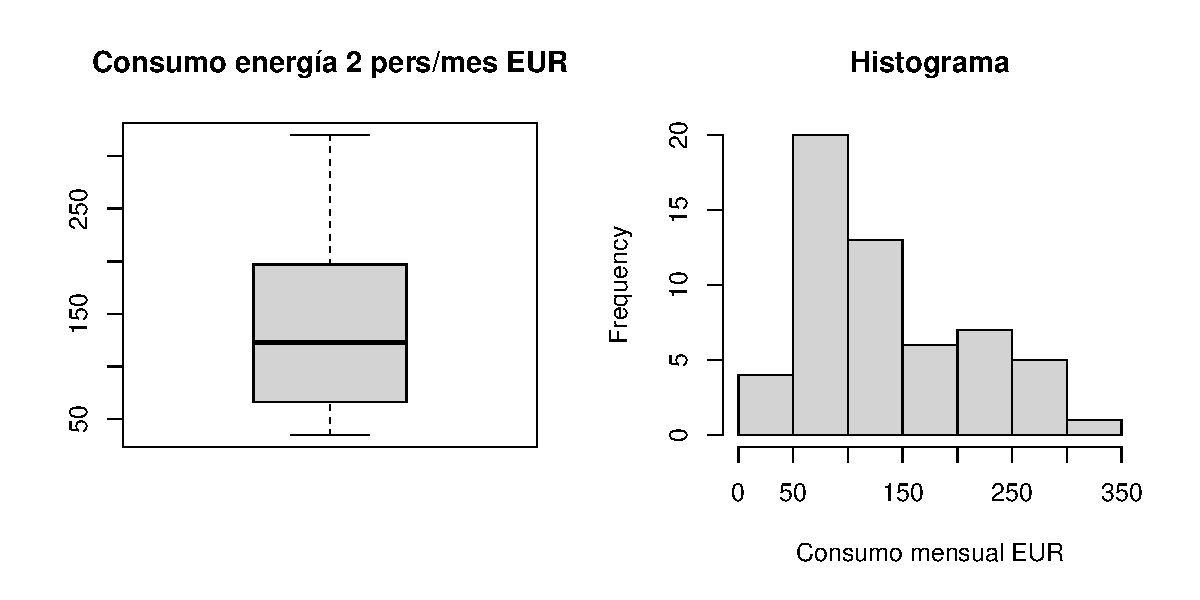
\includegraphics{PRA2_Data_cleaning_and_analysis_files/figure-latex/unnamed-chunk-11-1.pdf}

\begin{Shaded}
\begin{Highlighting}[]
\CommentTok{\# Outliers item: Monthly rent for 85 m2 (900 sqft) furnished accommodation in normal area}
\FunctionTok{par}\NormalTok{(}\AttributeTok{mfrow=}\FunctionTok{c}\NormalTok{(}\DecValTok{1}\NormalTok{,}\DecValTok{2}\NormalTok{))}
\NormalTok{df\_b}\OtherTok{\textless{}{-}}\FunctionTok{subset}\NormalTok{(df\_countries, }
\NormalTok{             Items }\SpecialCharTok{==} \StringTok{"Monthly rent for 85 m2 (900 sqft) furnished accommodation in normal area"}\NormalTok{)}
\FunctionTok{boxplot}\NormalTok{(df\_b}\SpecialCharTok{$}\NormalTok{EUR.Value, }\AttributeTok{main=}\StringTok{"Alquiler mensual EUR"}\NormalTok{)}
\FunctionTok{hist}\NormalTok{(df\_b}\SpecialCharTok{$}\NormalTok{EUR.Value, }\AttributeTok{main=}\StringTok{"Histograma"}\NormalTok{,}\AttributeTok{xlab=}\StringTok{"Alquiler mensual EUR"}\NormalTok{)}
\end{Highlighting}
\end{Shaded}

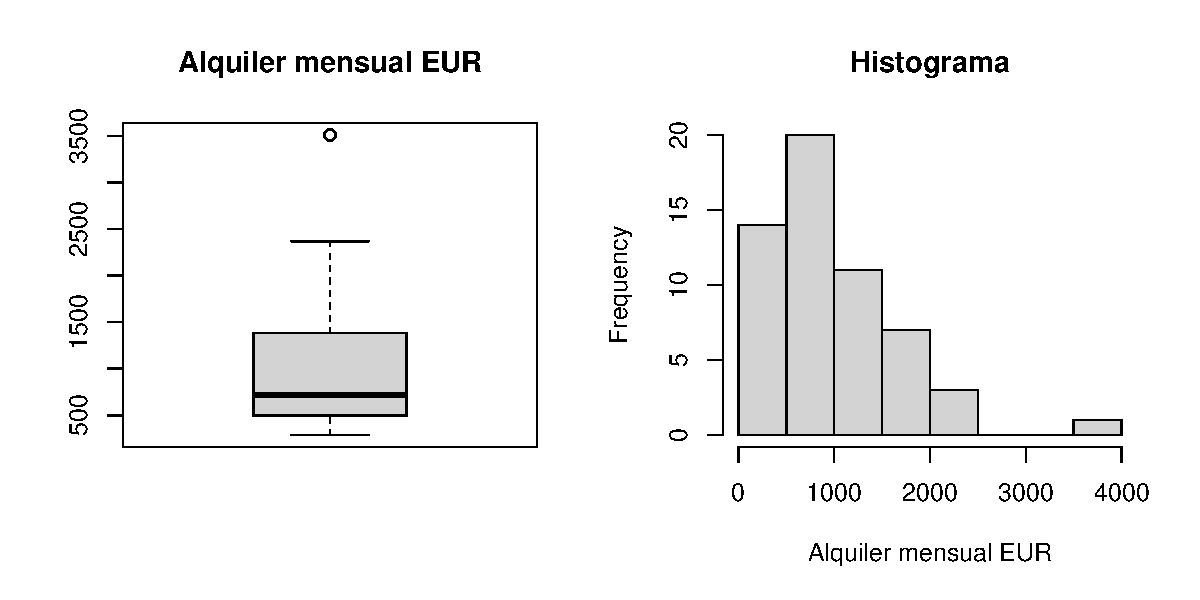
\includegraphics{PRA2_Data_cleaning_and_analysis_files/figure-latex/unnamed-chunk-11-2.pdf}

\begin{Shaded}
\begin{Highlighting}[]
\CommentTok{\# Outliers category: Food}
\FunctionTok{par}\NormalTok{(}\AttributeTok{mfrow=}\FunctionTok{c}\NormalTok{(}\DecValTok{1}\NormalTok{,}\DecValTok{2}\NormalTok{))}
\NormalTok{df\_c}\OtherTok{\textless{}{-}}\FunctionTok{subset}\NormalTok{(df\_countries, }
\NormalTok{             Category }\SpecialCharTok{==} \StringTok{"Food"}\NormalTok{)}
\FunctionTok{boxplot}\NormalTok{(df\_c}\SpecialCharTok{$}\NormalTok{EUR.Value, }\AttributeTok{main=}\StringTok{"Food"}\NormalTok{)}
\FunctionTok{hist}\NormalTok{(df\_c}\SpecialCharTok{$}\NormalTok{EUR.Value, }\AttributeTok{main=}\StringTok{"Histograma"}\NormalTok{,}\AttributeTok{xlab=}\StringTok{"Food"}\NormalTok{)}
\end{Highlighting}
\end{Shaded}

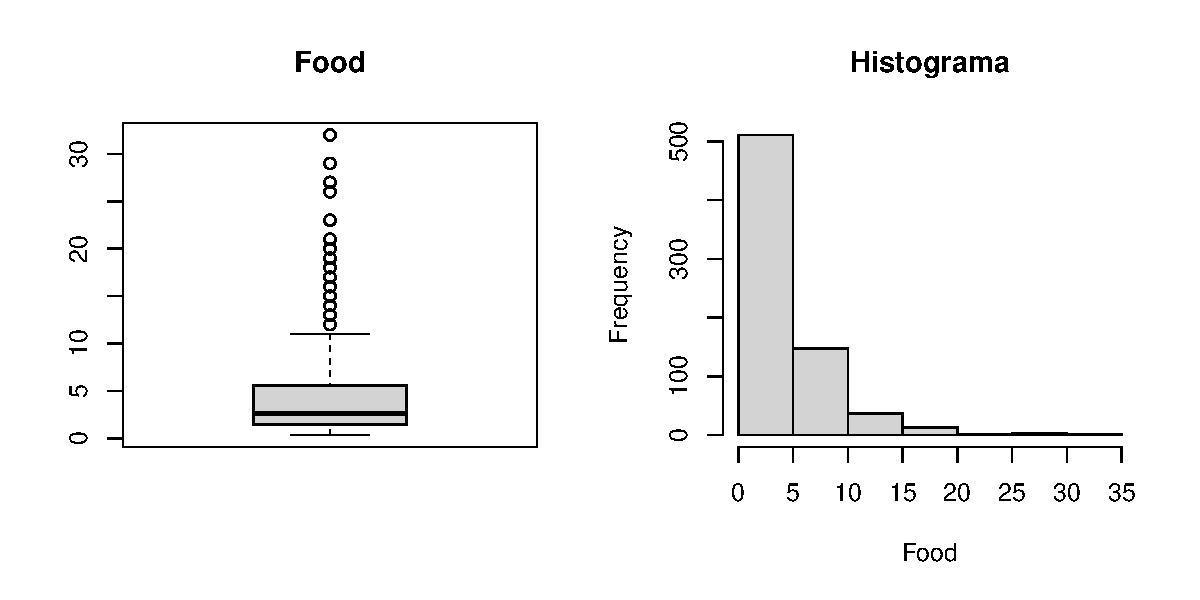
\includegraphics{PRA2_Data_cleaning_and_analysis_files/figure-latex/unnamed-chunk-11-3.pdf}

\begin{Shaded}
\begin{Highlighting}[]
\CommentTok{\# Outliers: SMI}
\FunctionTok{par}\NormalTok{(}\AttributeTok{mfrow=}\FunctionTok{c}\NormalTok{(}\DecValTok{1}\NormalTok{,}\DecValTok{2}\NormalTok{))}
\FunctionTok{boxplot}\NormalTok{(df\_countries}\SpecialCharTok{$}\NormalTok{SMI, }\AttributeTok{main=}\StringTok{"SMI EUR"}\NormalTok{)}
\FunctionTok{hist}\NormalTok{(df\_countries}\SpecialCharTok{$}\NormalTok{SMI, }\AttributeTok{main=}\StringTok{"Histograma"}\NormalTok{,}\AttributeTok{xlab=}\StringTok{"SMI EUR"}\NormalTok{)}
\end{Highlighting}
\end{Shaded}

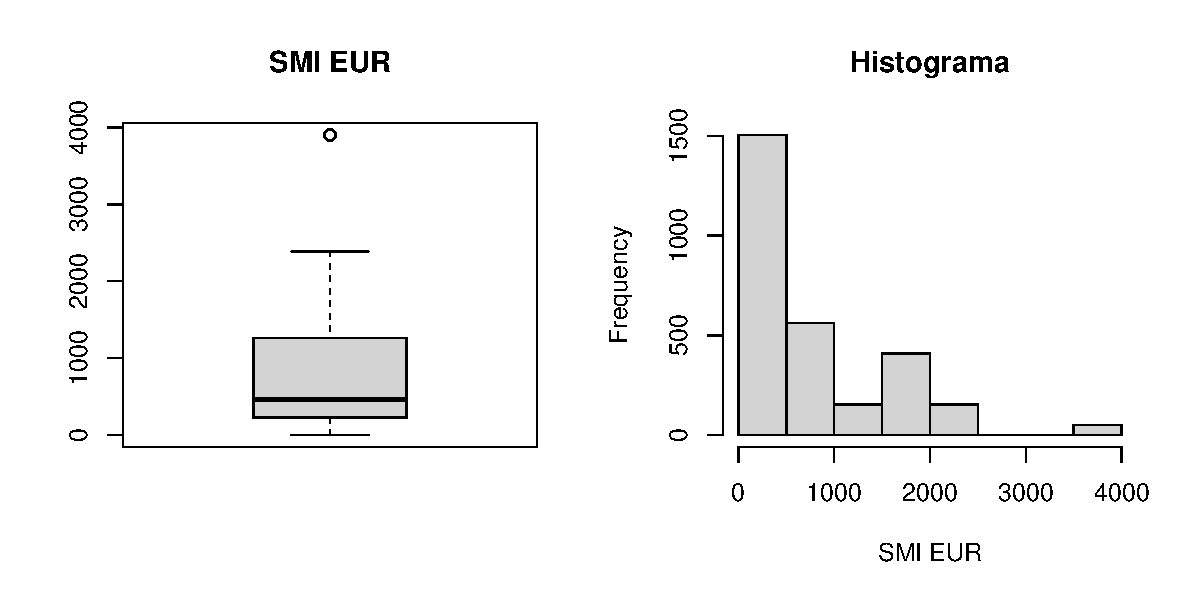
\includegraphics{PRA2_Data_cleaning_and_analysis_files/figure-latex/unnamed-chunk-11-4.pdf}

\begin{Shaded}
\begin{Highlighting}[]
\CommentTok{\# Outliers: PIB}
\FunctionTok{par}\NormalTok{(}\AttributeTok{mfrow=}\FunctionTok{c}\NormalTok{(}\DecValTok{1}\NormalTok{,}\DecValTok{2}\NormalTok{))}
\FunctionTok{boxplot}\NormalTok{(df\_countries}\SpecialCharTok{$}\NormalTok{PIB.anual, }\AttributeTok{main=}\StringTok{"PIB anual"}\NormalTok{)}
\FunctionTok{hist}\NormalTok{(df\_countries}\SpecialCharTok{$}\NormalTok{PIB.anual, }\AttributeTok{main=}\StringTok{"Histograma"}\NormalTok{,}\AttributeTok{xlab=}\StringTok{"PIB anual"}\NormalTok{)}
\end{Highlighting}
\end{Shaded}

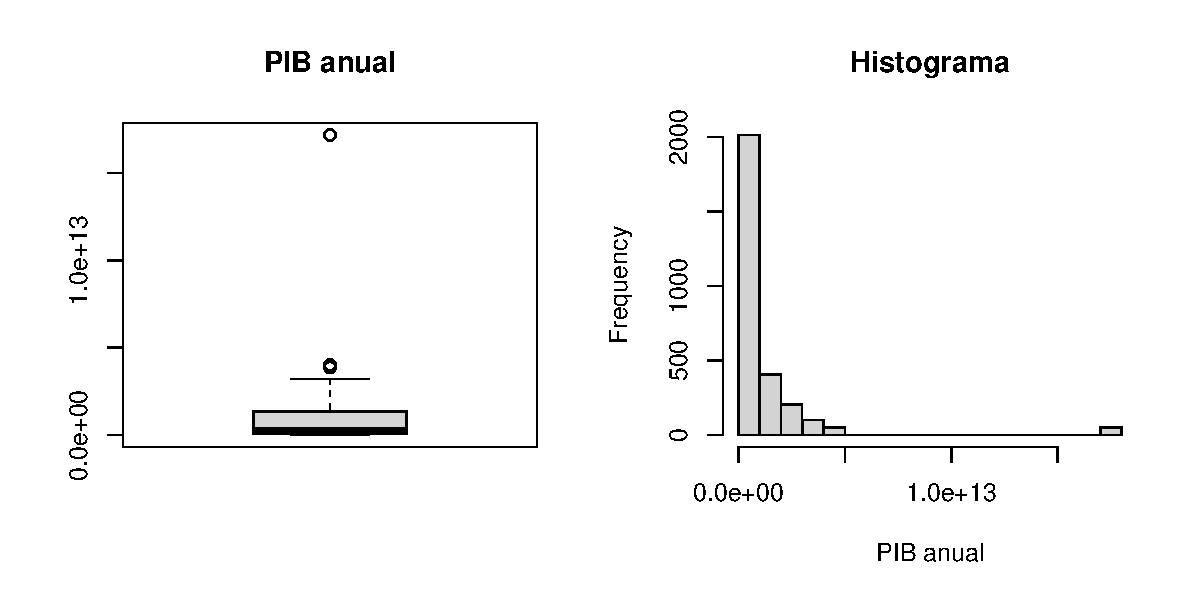
\includegraphics{PRA2_Data_cleaning_and_analysis_files/figure-latex/unnamed-chunk-11-5.pdf}

En las categorías anteriores podemos observar algunos \emph{outliers} a
considerar que pueden influir en el análisis.

\begin{Shaded}
\begin{Highlighting}[]
\CommentTok{\# Filtramos el dataset aplicando unas condiciones para cada Item}
\NormalTok{df\_countries }\OtherTok{\textless{}{-}} \FunctionTok{filter}\NormalTok{(df\_countries, Items\_factor }\SpecialCharTok{==} \DecValTok{42} \SpecialCharTok{\&}\NormalTok{ EUR.Value }\SpecialCharTok{\textless{}=} \DecValTok{2600} \SpecialCharTok{|}\NormalTok{ Items\_factor }\SpecialCharTok{!=} \DecValTok{42}\NormalTok{) }\CommentTok{\# Utilities}
\NormalTok{df\_countries }\OtherTok{\textless{}{-}} \FunctionTok{filter}\NormalTok{(df\_countries, Category }\SpecialCharTok{==} \StringTok{"Food"} \SpecialCharTok{\&}\NormalTok{ EUR.Value }\SpecialCharTok{\textless{}=} \DecValTok{10} \SpecialCharTok{|}\NormalTok{ Category }\SpecialCharTok{!=} \StringTok{"Food"}\NormalTok{) }\CommentTok{\#Food}
\NormalTok{df\_countries }\OtherTok{\textless{}{-}} \FunctionTok{filter}\NormalTok{(df\_countries, SMI }\SpecialCharTok{\textless{}=} \DecValTok{2500}\NormalTok{) }\CommentTok{\# SMI}
\NormalTok{df\_countries }\OtherTok{\textless{}{-}} \FunctionTok{filter}\NormalTok{(df\_countries, PIB.anual }\SpecialCharTok{\textless{}=} \FloatTok{1e13}\NormalTok{) }\CommentTok{\# PIB.anual}
\end{Highlighting}
\end{Shaded}

\hypertarget{guardamos-los-datos-pre-procesados}{%
\subsection{3. Guardamos los datos
pre-procesados}\label{guardamos-los-datos-pre-procesados}}

\begin{Shaded}
\begin{Highlighting}[]
\CommentTok{\# Guardamos los datos preprocesados en un fichero}
\FunctionTok{write.csv}\NormalTok{(df\_countries, }\StringTok{"../datasets/cost\_of\_living\_countries\_clean.csv"}\NormalTok{, }\AttributeTok{row.names =} \ConstantTok{FALSE}\NormalTok{)}
\end{Highlighting}
\end{Shaded}

\hypertarget{anuxe1lisis-de-los-datos}{%
\subsection{4. Análisis de los datos}\label{anuxe1lisis-de-los-datos}}

\hypertarget{datos-a-comparar.-valores-muxednimos-de-gasto-medio-por-categoruxeda.}{%
\subsubsection{4.1 Datos a comparar. Valores mínimos de gasto medio por
categoría.}\label{datos-a-comparar.-valores-muxednimos-de-gasto-medio-por-categoruxeda.}}

Con el objetivo de realizar un análisis generalizado del coste de vida
por países, vamos a generar un dataset con los promedios de gasto para
cada una de las 6 categorías que existen, independientemente del
\emph{Item}, para así poder realizar inferencia estadística (test de
hipótesis, estimación de parámetros, intervalos de confianza) entre las
distintas categorías o países.

\begin{Shaded}
\begin{Highlighting}[]
\CommentTok{\# Creamos el dataset con las columnas que usaremos}
\NormalTok{df\_countries\_2 }\OtherTok{\textless{}{-}}\NormalTok{ df\_countries[,}\FunctionTok{c}\NormalTok{(}\DecValTok{1}\NormalTok{,}\DecValTok{2}\NormalTok{,}\DecValTok{3}\NormalTok{,}\DecValTok{5}\NormalTok{,}\DecValTok{6}\NormalTok{,}\DecValTok{7}\NormalTok{)]}

\CommentTok{\# Agrupamos los datos y calculamos el valor medio de la columna EUR.Value}
\NormalTok{df\_countries\_avg }\OtherTok{\textless{}{-}} \FunctionTok{aggregate}\NormalTok{(df\_countries\_2}\SpecialCharTok{$}\NormalTok{EUR.Value, }\AttributeTok{by =} \FunctionTok{list}\NormalTok{(df\_countries\_2}\SpecialCharTok{$}\NormalTok{Ranking.position, }
\NormalTok{                                                                  df\_countries\_2}\SpecialCharTok{$}\NormalTok{Country,}
\NormalTok{                                                                  df\_countries\_2}\SpecialCharTok{$}\NormalTok{Category,}
\NormalTok{                                                                  df\_countries\_2}\SpecialCharTok{$}\NormalTok{PIB.anual,}
\NormalTok{                                                                  df\_countries\_2}\SpecialCharTok{$}\NormalTok{SMI), }
                              \AttributeTok{FUN =}\NormalTok{ mean)}

\FunctionTok{colnames}\NormalTok{(df\_countries\_avg) }\OtherTok{\textless{}{-}} \FunctionTok{c}\NormalTok{(}\StringTok{"Ranking.position"}\NormalTok{, }\StringTok{"Country"}\NormalTok{, }\StringTok{"Category"}\NormalTok{, }\StringTok{"PIB.anual"}\NormalTok{, }\StringTok{"SMI"}\NormalTok{, }\StringTok{"€.Avg.Expense"}\NormalTok{)}

\NormalTok{df\_countries\_summary }\OtherTok{\textless{}{-}} \FunctionTok{spread}\NormalTok{(df\_countries\_avg, }
\NormalTok{                                 Category, }
                                 \StringTok{\textasciigrave{}}\AttributeTok{€.Avg.Expense}\StringTok{\textasciigrave{}}\NormalTok{)}
\FunctionTok{str}\NormalTok{(df\_countries\_summary)}
\end{Highlighting}
\end{Shaded}

\begin{verbatim}
## 'data.frame':    54 obs. of  10 variables:
##  $ Ranking.position: int  5 6 7 11 12 13 14 15 16 17 ...
##  $ Country         : chr  "BAHAMAS" "HONG KONG" "IRELAND" "NETHERLANDS" ...
##  $ PIB.anual       : num  9.47e+09 3.12e+11 5.03e+11 9.41e+11 7.81e+10 ...
##  $ SMI             : num  804 734 1910 1934 2387 ...
##  $ Clothes         : num  97.5 52.2 75.8 80.5 84 ...
##  $ Entertainment   : num  139.5 64.1 85.4 98.8 42 ...
##  $ Food            : num  4.66 3.8 3.77 3.77 3.87 ...
##  $ Housing         : num  729 1059 816 721 801 ...
##  $ Personal Care   : num  20.95 8.23 14.43 12.21 10.83 ...
##  $ Transportation  : num  2911 13052 10437 9571 9847 ...
\end{verbatim}

Como ya hemos comentado, el objetivo de este dataset es poder realizar
una inferencia estadística sobre los distintos países o sobre la media
de gastos básicos en una categoría concreta. Debemos aclarar aquí, que
los valores almacenados para cada categoría \emph{no} indican el valor
medio de gasto en el país en cuestión para esa categoría, si no un
cálculo aproximado del valor medio que se podría gastar en cada
categoría si se realizara/adquiriese cada uno de los \emph{Items}
detallados en el conjunto de datos original. Es decir, que el gasto
medio de transporte en Bermuda sea 11714.35€, no quiere decir que se
gaste eso de media en transporte, pero sí consideramos el promedio de
comprar un coche, comprar un litro de gasolina y adquirir un abono
transporte. Debemos considerar estos valores como un indicador de la
categoría, y no como un gasto medio de la misma.

\hypertarget{normalidad-y-homogeneidad-de-la-varianza}{%
\subsubsection{4.2 Normalidad y Homogeneidad de la
varianza}\label{normalidad-y-homogeneidad-de-la-varianza}}

Evaluar la normalidad de los datos y la homogeneidad de las varianzas es
importante para asegurarnos de que los análisis estadísticos que
realizamos son válidos y que podemos interpretar los resultados de
manera adecuada. Estas evaluaciones nos permiten confirmar si los
supuestos necesarios para aplicar ciertas técnicas estadísticas se
cumplen. Si los datos no siguen una distribución normal o si las
varianzas no son similares entre grupos, es posible que los resultados
de nuestros análisis no sean confiables. Por lo tanto, al verificar la
normalidad de los datos y la homogeneidad de las varianzas, estamos
asegurándonos de que nuestras conclusiones se basen en fundamentos
sólidos y que nuestras inferencias y decisiones sean acertadas.

\hypertarget{normalidad}{%
\paragraph{4.2.1 Normalidad}\label{normalidad}}

\hypertarget{normalidad-de-las-variables-medias}{%
\subparagraph{4.2.1.1 Normalidad de las variables
medias}\label{normalidad-de-las-variables-medias}}

\hfill\break

Estudiemos la normalidad de las variables resultantes en el dataset con
los valores medios.

\begin{Shaded}
\begin{Highlighting}[]
\CommentTok{\# Normalidad: PIB.anual, Food, Clothes, Entertainment, Housing, SMI}
\FunctionTok{shapiro.test}\NormalTok{(df\_countries\_summary}\SpecialCharTok{$}\NormalTok{PIB.anual)}
\end{Highlighting}
\end{Shaded}

\begin{verbatim}
## 
##  Shapiro-Wilk normality test
## 
## data:  df_countries_summary$PIB.anual
## W = 0.73382, p-value = 1.476e-08
\end{verbatim}

\begin{Shaded}
\begin{Highlighting}[]
\FunctionTok{shapiro.test}\NormalTok{(df\_countries\_summary}\SpecialCharTok{$}\NormalTok{Food)}
\end{Highlighting}
\end{Shaded}

\begin{verbatim}
## 
##  Shapiro-Wilk normality test
## 
## data:  df_countries_summary$Food
## W = 0.85818, p-value = 1.361e-05
\end{verbatim}

\begin{Shaded}
\begin{Highlighting}[]
\FunctionTok{shapiro.test}\NormalTok{(df\_countries\_summary}\SpecialCharTok{$}\NormalTok{Clothes)}
\end{Highlighting}
\end{Shaded}

\begin{verbatim}
## 
##  Shapiro-Wilk normality test
## 
## data:  df_countries_summary$Clothes
## W = 0.9854, p-value = 0.7502
\end{verbatim}

\begin{Shaded}
\begin{Highlighting}[]
\FunctionTok{shapiro.test}\NormalTok{(df\_countries\_summary}\SpecialCharTok{$}\NormalTok{Entertainment)}
\end{Highlighting}
\end{Shaded}

\begin{verbatim}
## 
##  Shapiro-Wilk normality test
## 
## data:  df_countries_summary$Entertainment
## W = 0.96029, p-value = 0.071
\end{verbatim}

\begin{Shaded}
\begin{Highlighting}[]
\FunctionTok{shapiro.test}\NormalTok{(df\_countries\_summary}\SpecialCharTok{$}\NormalTok{Housing)}
\end{Highlighting}
\end{Shaded}

\begin{verbatim}
## 
##  Shapiro-Wilk normality test
## 
## data:  df_countries_summary$Housing
## W = 0.89048, p-value = 0.0001353
\end{verbatim}

\begin{Shaded}
\begin{Highlighting}[]
\FunctionTok{shapiro.test}\NormalTok{(df\_countries\_summary}\SpecialCharTok{$}\NormalTok{SMI)}
\end{Highlighting}
\end{Shaded}

\begin{verbatim}
## 
##  Shapiro-Wilk normality test
## 
## data:  df_countries_summary$SMI
## W = 0.82555, p-value = 1.75e-06
\end{verbatim}

Podemos comprobar que en los test anteriores, las variables:
\emph{PIB.anual}, \emph{Food}, \emph{Housing} y \emph{SMI} siguen
distribuciones normales mediante el test de \textbf{Shapiro-Wilk} con un
p-valor menor que un nivel de significancia \(\alpha=0.05\). En las
variables \emph{Entertainment} y \emph{Clothes} no podemos decir lo
mismo, a pesar de que en el caso de nuestra población, al ser una
muestra grande con n\textgreater30 podríamos asumir la hipótesis de
normalidad de las medias por el teorema del límite central.

\hypertarget{normalidad-de-la-variable-eur.value-para-el-item-monthly-rent-for-85-m2-900-sqft-furnished-accommodation-in-normal-area}{%
\subparagraph{\texorpdfstring{4.2.1.2 Normalidad de la variable
EUR.Value para el Item: Monthly rent for \(85 m^{2}\) (900 sqft)
furnished accommodation in normal
area}{4.2.1.2 Normalidad de la variable EUR.Value para el Item: Monthly rent for 85 m\^{}\{2\} (900 sqft) furnished accommodation in normal area}}\label{normalidad-de-la-variable-eur.value-para-el-item-monthly-rent-for-85-m2-900-sqft-furnished-accommodation-in-normal-area}}

\hfill\break

Ahora comprobaremos la normalidad para la variable \emph{EUR.value} para
el \emph{Item} que querremos estudiar en los próximos análisis:

\begin{Shaded}
\begin{Highlighting}[]
\CommentTok{\# Recogemos las filas que traten sombre este Item}
\NormalTok{df\_countries\_test }\OtherTok{\textless{}{-}} \FunctionTok{filter}\NormalTok{(df\_countries, Items }\SpecialCharTok{==} \StringTok{"Monthly rent for 85 m2 (900 sqft) furnished accommodation in normal area"}\NormalTok{)}

\CommentTok{\# Normalidad: EUR.Value}
\FunctionTok{shapiro.test}\NormalTok{(df\_countries\_test}\SpecialCharTok{$}\NormalTok{EUR.Value)}
\end{Highlighting}
\end{Shaded}

\begin{verbatim}
## 
##  Shapiro-Wilk normality test
## 
## data:  df_countries_test$EUR.Value
## W = 0.88564, p-value = 0.0001084
\end{verbatim}

Como se puede observar, el p-value resultante es menor al valor de
significancia \(\alpha=0.05\), indicando normalidad en la variable.

\hypertarget{homocedasticidad}{%
\paragraph{4.2.2 Homocedasticidad}\label{homocedasticidad}}

\hfill\break

Comprobemos si la variable \emph{EUR.Value} cumple la igualdad de
varianzas entre dos grupos a comparar para poder aplicar contraste de
hipótesis a los datos. Para ello, escogeremos dos Items similares que
queremos estudiar y aplicaremos el Test de Levene:

\begin{itemize}
\tightlist
\item
  ``Monthly rent for 85 m2 (900 sqft) furnished accommodation in normal
  area''
\item
  ``Monthly rent for 85 m2 (900 sqft) furnished accommodation in
  expensive area''
\end{itemize}

\begin{Shaded}
\begin{Highlighting}[]
\CommentTok{\# Conseguimos los dos grupos de los cuales queremos estudiar su homogeneidad de varianzas}
\NormalTok{df\_countries\_homocedasticidad }\OtherTok{\textless{}{-}} \FunctionTok{filter}\NormalTok{(df\_countries, Items  }\SpecialCharTok{\%in\%} \FunctionTok{c}\NormalTok{(}\StringTok{"Monthly rent for 85 m2 (900 sqft) furnished accommodation in normal area"}\NormalTok{, }\StringTok{"Monthly rent for 85 m2 (900 sqft) furnished accommodation in expensive area"}\NormalTok{))}

\CommentTok{\# Homocedasticidad: EUR.Value en función de Items}
\FunctionTok{leveneTest}\NormalTok{(}\AttributeTok{y =}\NormalTok{ df\_countries\_homocedasticidad}\SpecialCharTok{$}\NormalTok{EUR.Value, }\AttributeTok{group =}\NormalTok{ df\_countries\_homocedasticidad}\SpecialCharTok{$}\NormalTok{Items, }\AttributeTok{center =} \StringTok{"median"}\NormalTok{)}
\end{Highlighting}
\end{Shaded}

\begin{verbatim}
## Levene's Test for Homogeneity of Variance (center = "median")
##        Df F value Pr(>F)
## group   1  2.4585 0.1199
##       105
\end{verbatim}

Para estos resultados del \textbf{Test de Levene}, podemos observar que
su \(p-value=0.1199\) resultante es mayor al nivel de significancia
\(\alpha=0.05\). Por ende, no tenemos pruebas suficientes como para
rechazar la hipótesis nula, es decir, las varianzas no difieren
significativamente entre ellas y podemos asumir homogeneidad de varianza
entre los 2 grupos de alquiler.

\hypertarget{pruebas-estaduxedsticas}{%
\subsubsection{4.3 Pruebas estadísticas}\label{pruebas-estaduxedsticas}}

\hfill\break
Dentro de todas las pruebas estadísticas que hay, nos hemos decantado
por aquellas que nos ayudarán a resolver las preguntas planteadas en el
apartado uno: el contraste de hipótesis, la regresión lineal y la
regresión logística.

\hypertarget{contraste-de-hipuxf3tesis}{%
\paragraph{4.3.2 Contraste de
hipótesis}\label{contraste-de-hipuxf3tesis}}

\hfill\break

Queremos estudiar si un alquiler en una zona normal, es decir, el
\emph{Item} ``Monthly rent for 85 m2 (900 sqft) furnished accommodation
in normal area'' es significativamente mayor en Europa que en América.
Para ello, lo mejor es hacer un contraste de hipótesis al 95\% de
confianza. Por ende, podemos establecer las siguientes hipótesis nula
\(H_{0}\) y alternativa \(H_{1}\):

\(H_{0}: \theta_{0}=\theta_{1}\)\\
\(H_{1}: \theta_{0}>\theta_{1}\)

En este caso tendremos que:

\begin{enumerate}
\def\labelenumi{\arabic{enumi}.}
\item
  \(H_{0}\) establece que ``la media del alquiler mensual en un zona
  normal en Europa es \textbf{igual} que la misma en América''.
\item
  \(H_{1}\), ``la media del alquiler mensual en un zona normal en Europa
  es \textbf{mayor} que en América''.
\item
  \(\theta_{0}\) es el valor monetario medio en euros del alquiler en
  Europa.
\item
  \(\theta_{1}\) es el valor monetario medio en euros del alquiler en
  América.
\end{enumerate}

Para este estudio, realizaremos un \textbf{contraste de dos muestras
independientes sobre la media con varianzas conocidas}, siendo esta
muestras independientes \(\theta_{0}\) y \(\theta_{1}\). La idea es
refutar la hipótesis nula basándonos en evidencia positiva y superior al
umbral de aceptación establecido: a base de test con un nivel de
confianza del 95\%.

Usaremos este tipo de contraste ya que la pregunta nos plantea dos
muestras que definiremos uniformemente, es decir, escogeremos 5 países
de cada continente para conformar sus muestras. De estas mismas, podemos
calcular su media sabiendo el número de países involucrados y, por ende,
su varianza será conocida. El procedimiento a seguir será aplicar el
\textbf{Teorema del Límite Central} para intentar rechazar la hipótesis
nula. De esta forma, comenzaremos por un test unilateral por la derecha,
donde la zona de aceptación de la hipótesis nula estará comprendida
entre (-∞, \(z_{1-∞}\){]}:

\begin{Shaded}
\begin{Highlighting}[]
\CommentTok{\# Definimos la función para calcular el valor observado, el valor crítico y el valor p}
\NormalTok{def\_valores\_alquiler }\OtherTok{\textless{}{-}} \ControlFlowTok{function}\NormalTok{(theta\_0, theta\_1, alpha) \{}
    \CommentTok{\# Primero conseguimos la media y la varianza de cada muestra}
\NormalTok{    alquiler\_mean\_EUR }\OtherTok{\textless{}{-}} \FunctionTok{mean}\NormalTok{(theta\_0)}
\NormalTok{    alquiler\_mean\_AME }\OtherTok{\textless{}{-}} \FunctionTok{mean}\NormalTok{(theta\_1)}
\NormalTok{    alquiler\_var\_EUR }\OtherTok{\textless{}{-}} \FunctionTok{var}\NormalTok{(theta\_0, }\AttributeTok{na.rm =} \ConstantTok{TRUE}\NormalTok{)}
\NormalTok{    alquiler\_var\_AME }\OtherTok{\textless{}{-}} \FunctionTok{var}\NormalTok{(theta\_1, }\AttributeTok{na.rm =} \ConstantTok{TRUE}\NormalTok{)}
    
    \CommentTok{\# Luego calculamos el valor observado}
\NormalTok{    n\_EUR }\OtherTok{\textless{}{-}} \FunctionTok{length}\NormalTok{(theta\_0)}
\NormalTok{    n\_AME }\OtherTok{\textless{}{-}} \FunctionTok{length}\NormalTok{(theta\_1)}
\NormalTok{    valor\_obs }\OtherTok{\textless{}{-}}\NormalTok{ (alquiler\_mean\_EUR }\SpecialCharTok{{-}}\NormalTok{ alquiler\_mean\_AME) }\SpecialCharTok{/} \FunctionTok{sqrt}\NormalTok{(alquiler\_var\_EUR }\SpecialCharTok{/}\NormalTok{ n\_EUR }\SpecialCharTok{+}\NormalTok{ alquiler\_var\_AME }\SpecialCharTok{/}\NormalTok{ n\_AME) }
    
    \CommentTok{\# Calculamos el valor crítico}
\NormalTok{    valor\_crit }\OtherTok{\textless{}{-}} \FunctionTok{qnorm}\NormalTok{(alpha, }\AttributeTok{lower.tail =} \ConstantTok{FALSE}\NormalTok{) }
    
    \CommentTok{\# Calcular el valor p}
\NormalTok{    valor\_p }\OtherTok{\textless{}{-}} \FunctionTok{pnorm}\NormalTok{(valor\_obs, }\AttributeTok{lower.tail =} \ConstantTok{FALSE}\NormalTok{) }
    
    \CommentTok{\# Devolvemos los valores obtenidos}
    \FunctionTok{return}\NormalTok{(}\FunctionTok{c}\NormalTok{(valor\_obs, valor\_crit, valor\_p)) }
\NormalTok{\}}
\CommentTok{\# Primero definiremos las muestras}
\NormalTok{df\_Europa }\OtherTok{\textless{}{-}} \FunctionTok{subset}\NormalTok{(df\_countries, }
\NormalTok{                    Items }\SpecialCharTok{==} \StringTok{"Monthly rent for 85 m2 (900 sqft) furnished accommodation in normal area"} 
                    \SpecialCharTok{\&}\NormalTok{ Country }\SpecialCharTok{\%in\%} \FunctionTok{c}\NormalTok{(}\StringTok{"FRANCE"}\NormalTok{, }\StringTok{"ITALY"}\NormalTok{, }\StringTok{"FINLAND"}\NormalTok{, }\StringTok{"SWITZERLAND"}\NormalTok{, }\StringTok{"GERMANY"}\NormalTok{)) }
\NormalTok{df\_America }\OtherTok{\textless{}{-}} \FunctionTok{subset}\NormalTok{(df\_countries, }
\NormalTok{                    Items }\SpecialCharTok{==} \StringTok{"Monthly rent for 85 m2 (900 sqft) furnished accommodation in normal area"} 
                    \SpecialCharTok{\&}\NormalTok{ Country }\SpecialCharTok{\%in\%} \FunctionTok{c}\NormalTok{(}\StringTok{"UNITED STATES"}\NormalTok{, }\StringTok{"MEXICO"}\NormalTok{, }\StringTok{"CANADA"}\NormalTok{, }\StringTok{"URUGUAY"}\NormalTok{, }\StringTok{"BOLIVIA"}\NormalTok{)) }

\CommentTok{\# Calculamos los valores al 95\% de confianza y lo mostramos por pantalla}
\NormalTok{valores\_alquiler }\OtherTok{\textless{}{-}} \FunctionTok{def\_valores\_alquiler}\NormalTok{(df\_Europa}\SpecialCharTok{$}\NormalTok{EUR.Value, df\_America}\SpecialCharTok{$}\NormalTok{EUR.Value, }\FloatTok{0.05}\NormalTok{)}
\FunctionTok{cat}\NormalTok{(}\StringTok{"El valor observado: "}\NormalTok{, valores\_alquiler[}\DecValTok{1}\NormalTok{],}
    \StringTok{"}\SpecialCharTok{\textbackslash{}n}\StringTok{El valor crítico: "}\NormalTok{, valores\_alquiler[}\DecValTok{2}\NormalTok{],}
    \StringTok{"}\SpecialCharTok{\textbackslash{}n}\StringTok{El valor p al 95\%: "}\NormalTok{, valores\_alquiler[}\DecValTok{3}\NormalTok{], }\StringTok{""}\NormalTok{)}
\end{Highlighting}
\end{Shaded}

\begin{verbatim}
## El valor observado:  2.964443 
## El valor crítico:  1.644854 
## El valor p al 95%:  0.001516159
\end{verbatim}

\hypertarget{regresiuxf3n-lineal}{%
\paragraph{4.3.1 Regresión lineal}\label{regresiuxf3n-lineal}}

\hfill\break

En este apartado vamos a realizar una regresión lineal para estudiar el
\emph{SMI} de un país en función de los valores medios de las categorías
que siguen una distribución normal: \emph{Food}, \emph{Housing},
\emph{PIB.anual}. De esta forma, a partir de los valores medios de
gastos mínimos (recordamos que el dataset no guarda los valores medios
de gasto, si no una muestra de gasto mínimo) en un país determinado,
podremos dar respuesta a la pregunta 2.

\begin{Shaded}
\begin{Highlighting}[]
\CommentTok{\# Generamos el modelo lineal}
\NormalTok{model\_SMI }\OtherTok{\textless{}{-}} \FunctionTok{lm}\NormalTok{(SMI }\SpecialCharTok{\textasciitilde{}}\NormalTok{ Food }\SpecialCharTok{+}\NormalTok{ Housing }\SpecialCharTok{+}\NormalTok{ PIB.anual, }\AttributeTok{data =}\NormalTok{ df\_countries\_summary)}
\FunctionTok{summary}\NormalTok{(model\_SMI)}
\end{Highlighting}
\end{Shaded}

\begin{verbatim}
## 
## Call:
## lm(formula = SMI ~ Food + Housing + PIB.anual, data = df_countries_summary)
## 
## Residuals:
##      Min       1Q   Median       3Q      Max 
## -1228.17  -242.05    39.31   213.85  1061.40 
## 
## Coefficients:
##               Estimate Std. Error t value Pr(>|t|)    
## (Intercept) -4.572e+02  2.798e+02  -1.634 0.108526    
## Food         7.340e+01  9.415e+01   0.780 0.439308    
## Housing      1.954e+00  3.733e-01   5.235 3.29e-06 ***
## PIB.anual    2.265e-10  6.164e-11   3.675 0.000581 ***
## ---
## Signif. codes:  0 '***' 0.001 '**' 0.01 '*' 0.05 '.' 0.1 ' ' 1
## 
## Residual standard error: 456.2 on 50 degrees of freedom
## Multiple R-squared:  0.5852, Adjusted R-squared:  0.5603 
## F-statistic: 23.51 on 3 and 50 DF,  p-value: 1.239e-09
\end{verbatim}

Si queremos interpretar la calidad del ajuste de este modelo, debemos
estudiar el \textbf{Coeficiente de Determinación} \(R^2\), que consiste
en la proporción de variabilidad explicada por el modelo con respecto a
la variabilidad total. Lo que buscaremos es que este coeficiente se
aproxime lo máximo a 1, ya que indicará que el modelo hace un buen
ajuste. Dentro del \emph{summary} del modelo, lo podremos encontrar bajo
el nombre ``Multiple R-squared'' y es 0.5852. Esto nos muestra que el
58.52\% de la variable dependiente \textbf{SMI} puede ser explicada por
las variables independientes \textbf{Food}, \textbf{Housing} y
\textbf{PIB.anual}.

Por otro lado, observamos que solo las categorías \emph{Housing} y
\emph{PIB.anual} tienen una influencia significante en la definición del
salario mínimo de un país ya que su \emph{p-value} es menor al nivel de
significancia \(\alpha=0.05\). sin embargo, no podemos decir los mismo
de la categoría \emph{Food}, al menos con los datos recogidos en nuestro
dataset. Esto nos explica por que el \(R^2\) llega solo a casi el 60\%:
faltan más variables para completar el concepto del \emph{SMI}, aunque
es un ajuste bastante decente y que puede dar resultados.

\hypertarget{regresiuxf3n-loguxedstica}{%
\paragraph{4.3.2 Regresión logística}\label{regresiuxf3n-loguxedstica}}

\hfill\break

Para poder empezar el último análisis estadístico, crearemos una nueva
variable dicotómica para ser nuestra variable dependiente: SMI\_bin.
Esta nueva variable está relacionada con los valores de la variable
\textbf{SMI} y se codificará de la siguiente forma: ``1'', para valores
de \textbf{SMI} superiores al SMI de España, y ``0'' con valores de
\textbf{SMI} inferiores al de España. Vamos a crearla:

\begin{Shaded}
\begin{Highlighting}[]
\CommentTok{\#Extraemos el SMI de España}
\NormalTok{SMI\_españa }\OtherTok{\textless{}{-}}\NormalTok{ df\_countries\_summary}\SpecialCharTok{$}\NormalTok{SMI[df\_countries\_summary}\SpecialCharTok{$}\NormalTok{Country }\SpecialCharTok{==} \StringTok{"SPAIN"}\NormalTok{]}

\CommentTok{\# Crearemos la nueva variable dicotómica SMI\_bin}
\NormalTok{df\_countries\_summary}\SpecialCharTok{$}\NormalTok{SMI\_bin }\OtherTok{\textless{}{-}} \FunctionTok{ifelse}\NormalTok{(df\_countries\_summary}\SpecialCharTok{$}\NormalTok{SMI }\SpecialCharTok{\textgreater{}}\NormalTok{ SMI\_españa, }\DecValTok{1}\NormalTok{, }\DecValTok{0}\NormalTok{)}
\end{Highlighting}
\end{Shaded}

Dado que queremos definir un modelo de regresión logística, el siguiente
paso es separar los datos en dos conjuntos aleatorios: el conjunto de
entrenamiento (training, 80\% de los datos) y el conjunto de prueba
(testing, 20\% de los datos). Esto nos ayudará a estimar de forma más
objetiva la precisión del modelo. Por ende, ajustaremos el modelo con el
conjunto de entrenamiento, y evaluaremos la precisión con el conjunto de
prueba.

\begin{Shaded}
\begin{Highlighting}[]
\CommentTok{\# Fijaremos una semilla aleatoria para reproducibilidad}
\FunctionTok{set.seed}\NormalTok{(}\DecValTok{27}\NormalTok{)}

\CommentTok{\# Dividiremos el conjunto de datos original en conjuntos de entrenamiento y prueba}
\NormalTok{train\_test }\OtherTok{\textless{}{-}} \FunctionTok{createDataPartition}\NormalTok{(df\_countries\_summary}\SpecialCharTok{$}\NormalTok{SMI\_bin, }\AttributeTok{p =} \FloatTok{0.80}\NormalTok{ , }\AttributeTok{list =} \ConstantTok{FALSE}\NormalTok{)}

\CommentTok{\# Para ello nos quedaremos como Train las filas del conjunto de datos que pertenezcan a la partición }
\NormalTok{train\_dataset }\OtherTok{\textless{}{-}}\NormalTok{ df\_countries\_summary[train\_test, ]}

\CommentTok{\# Y dejaremos el resto como Test}
\NormalTok{test\_dataset }\OtherTok{\textless{}{-}}\NormalTok{ df\_countries\_summary[}\SpecialCharTok{{-}}\NormalTok{train\_test, ]}
\end{Highlighting}
\end{Shaded}

Dado que la categoría \emph{Food} no ayudaba al modelo lineal, para el
modelo logístico la hemos intercambiado por \emph{Clothes} para estudiar
si ayuda al ajuste de la nueva variable \emph{SMI\_re} o no:

\begin{Shaded}
\begin{Highlighting}[]
\CommentTok{\# Definiremos el modelo logístico con SMI\_bin como variable dependiente y las categorías y el PIB, como independientes}
\NormalTok{modelo\_SMI\_bin }\OtherTok{\textless{}{-}} \FunctionTok{glm}\NormalTok{(SMI\_bin }\SpecialCharTok{\textasciitilde{}}\NormalTok{ PIB.anual }\SpecialCharTok{+}\NormalTok{ Clothes }\SpecialCharTok{+}\NormalTok{ Housing, train\_dataset, }\AttributeTok{family =}\NormalTok{ binomial)}

\CommentTok{\# Mostraremos los valores resultantes}
\FunctionTok{summary}\NormalTok{(modelo\_SMI\_bin)}
\end{Highlighting}
\end{Shaded}

\begin{verbatim}
## 
## Call:
## glm(formula = SMI_bin ~ PIB.anual + Clothes + Housing, family = binomial, 
##     data = train_dataset)
## 
## Deviance Residuals: 
##      Min        1Q    Median        3Q       Max  
## -2.13042  -0.24267  -0.10314  -0.01784   1.65898  
## 
## Coefficients:
##               Estimate Std. Error z value Pr(>|z|)   
## (Intercept) -1.617e+01  5.560e+00  -2.908  0.00363 **
## PIB.anual    1.610e-12  6.506e-13   2.474  0.01335 * 
## Clothes      1.351e-01  5.783e-02   2.336  0.01950 * 
## Housing      7.062e-03  3.217e-03   2.195  0.02815 * 
## ---
## Signif. codes:  0 '***' 0.001 '**' 0.01 '*' 0.05 '.' 0.1 ' ' 1
## 
## (Dispersion parameter for binomial family taken to be 1)
## 
##     Null deviance: 47.164  on 43  degrees of freedom
## Residual deviance: 18.567  on 40  degrees of freedom
## AIC: 26.567
## 
## Number of Fisher Scoring iterations: 7
\end{verbatim}

A diferencia de \emph{Food}, el p-value de \emph{Clothes} es menor al
valor de significancia \(\alpha=0.05\). Por ende, se debería tener en
cuenta junto con \emph{Housing} y \emph{PIB.anual} que también cumplen
la condición. Por otro lado, al ser un modelo de regresión de logística,
el valor que debemos estudiar es el AIC: cuanto más cerca del 0, mejor
se ajusta el modelo a los datos aportados. Como vemos el \(AIC=26.567\)
es bastante cercano a cero, indicando un buen ajuste.

Ahora analizaremos dicho ajuste con el conjunto de validación. Para
ello, predeciremos las etiquetas de \emph{SMI\_bin} para los valores
restantes y estudiaremos tanto su matriz de confusión como su curva ROC:

\begin{Shaded}
\begin{Highlighting}[]
\CommentTok{\# Extraemos las predicciones del modelo para el conjunto de datos de testing}
\NormalTok{predicciones }\OtherTok{\textless{}{-}} \FunctionTok{predict}\NormalTok{(modelo\_SMI\_bin, }\AttributeTok{newdata =}\NormalTok{ test\_dataset, }\AttributeTok{type =} \StringTok{"response"}\NormalTok{)}

\CommentTok{\# Dado que queremos estar seguros de nuestra predicción,}
\CommentTok{\# discretizamos dichas predicciones en función de su valor: }
\CommentTok{\#   {-} 1 si el valor es mayor o igual a 0.80}
\CommentTok{\#   {-} 0 si el valor es menor a 0.80}
\NormalTok{y\_pred }\OtherTok{\textless{}{-}} \FunctionTok{ifelse}\NormalTok{(predicciones }\SpecialCharTok{\textgreater{}=} \FloatTok{0.8}\NormalTok{, }\DecValTok{1}\NormalTok{, }\DecValTok{0}\NormalTok{)}

\CommentTok{\# Calculamos la matriz de confusión}
\NormalTok{matriz\_confusion }\OtherTok{\textless{}{-}} \FunctionTok{confusionMatrix}\NormalTok{(}\FunctionTok{factor}\NormalTok{(y\_pred), }\FunctionTok{factor}\NormalTok{(test\_dataset}\SpecialCharTok{$}\NormalTok{SMI\_bin), }\AttributeTok{dnn =} \FunctionTok{c}\NormalTok{(}\StringTok{"Prediction"}\NormalTok{, }\StringTok{"Reference"}\NormalTok{))}

\CommentTok{\# Preparamos el plot para enseñar la matriz de confusión}
\NormalTok{plt }\OtherTok{\textless{}{-}} \FunctionTok{as.data.frame}\NormalTok{(matriz\_confusion}\SpecialCharTok{$}\NormalTok{table)}
\NormalTok{plt}\SpecialCharTok{$}\NormalTok{Prediction }\OtherTok{\textless{}{-}} \FunctionTok{factor}\NormalTok{(plt}\SpecialCharTok{$}\NormalTok{Prediction, }\AttributeTok{levels =} \FunctionTok{rev}\NormalTok{(}\FunctionTok{levels}\NormalTok{(plt}\SpecialCharTok{$}\NormalTok{Prediction)))}
\NormalTok{plt}\SpecialCharTok{$}\NormalTok{Reference }\OtherTok{\textless{}{-}} \FunctionTok{factor}\NormalTok{(plt}\SpecialCharTok{$}\NormalTok{Reference, }\AttributeTok{levels =} \FunctionTok{rev}\NormalTok{(}\FunctionTok{levels}\NormalTok{(plt}\SpecialCharTok{$}\NormalTok{Reference)))}

\FunctionTok{ggplot}\NormalTok{(plt, }\FunctionTok{aes}\NormalTok{(Prediction, Reference, }\AttributeTok{fill =}\NormalTok{ Freq)) }\SpecialCharTok{+}
       \FunctionTok{geom\_tile}\NormalTok{() }\SpecialCharTok{+}
       \FunctionTok{geom\_text}\NormalTok{(}\FunctionTok{aes}\NormalTok{(}\AttributeTok{label =}\NormalTok{ Freq)) }\SpecialCharTok{+}
       \FunctionTok{scale\_fill\_gradient}\NormalTok{(}\AttributeTok{low =} \StringTok{"white"}\NormalTok{, }\AttributeTok{high =} \StringTok{"\#197376"}\NormalTok{) }\SpecialCharTok{+}
       \FunctionTok{labs}\NormalTok{(}\AttributeTok{x =} \StringTok{"Prediction"}\NormalTok{, }\AttributeTok{y =} \StringTok{"Reference"}\NormalTok{) }\SpecialCharTok{+}
       \FunctionTok{scale\_x\_discrete}\NormalTok{(}\AttributeTok{labels =} \FunctionTok{levels}\NormalTok{(plt}\SpecialCharTok{$}\NormalTok{Prediction)) }\SpecialCharTok{+}
       \FunctionTok{scale\_y\_discrete}\NormalTok{(}\AttributeTok{labels =} \FunctionTok{levels}\NormalTok{(plt}\SpecialCharTok{$}\NormalTok{Reference))}
\end{Highlighting}
\end{Shaded}

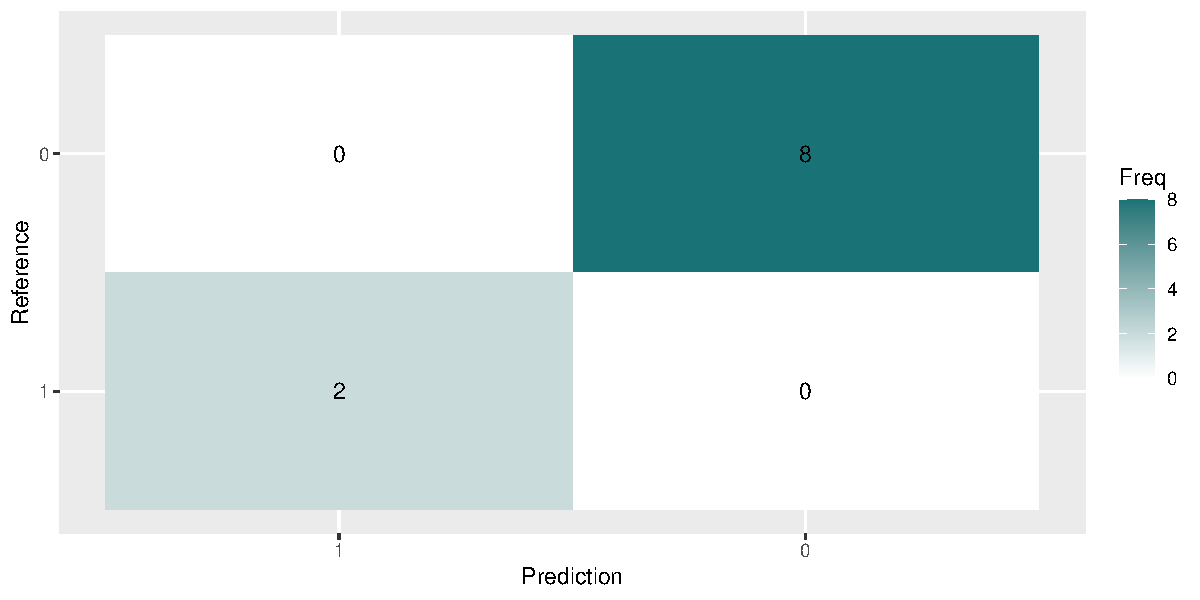
\includegraphics{PRA2_Data_cleaning_and_analysis_files/figure-latex/unnamed-chunk-23-1.pdf}

\begin{Shaded}
\begin{Highlighting}[]
\CommentTok{\# Mostramos los resultados}
\FunctionTok{cat}\NormalTok{(}\StringTok{"Sensibilidad: "}\NormalTok{, }\FunctionTok{round}\NormalTok{(matriz\_confusion}\SpecialCharTok{$}\NormalTok{byClass[}\StringTok{"Sensitivity"}\NormalTok{], }\DecValTok{4}\NormalTok{))}
\end{Highlighting}
\end{Shaded}

\begin{verbatim}
## Sensibilidad:  1
\end{verbatim}

\begin{Shaded}
\begin{Highlighting}[]
\FunctionTok{cat}\NormalTok{(}\StringTok{"Especificidad: "}\NormalTok{, }\FunctionTok{round}\NormalTok{(matriz\_confusion}\SpecialCharTok{$}\NormalTok{byClass[}\StringTok{"Specificity"}\NormalTok{], }\DecValTok{4}\NormalTok{))}
\end{Highlighting}
\end{Shaded}

\begin{verbatim}
## Especificidad:  1
\end{verbatim}

Observando estos resultados, el modelo funciona excelentemente bien para
el desbalanceo que hay entre las etiquetas ``superior al SMI de España''
(predicción \(\geq\) 0.80) y las etiquetas de ``inferior al SMI de
España'' (predicción \textless{} 0.80). Este desajuste en la cantidad de
datos por clase siempre puede causar problemas en el entrenamiento de
modelos y en su posterior evaluación. Sin embargo, su especificidad y su
sensibilidad son redondas, convirtiéndose en un excelente modelo de
regresión logística.

Por último, enseñaremos la gráfica de la curva ROC y junto con el área
debajo de la curva (AUC):

\begin{Shaded}
\begin{Highlighting}[]
\CommentTok{\# Crearemos la instancia del objeto de la curva ROC y extraeremos sus valores}
\NormalTok{roc }\OtherTok{\textless{}{-}} \FunctionTok{roc}\NormalTok{(test\_dataset}\SpecialCharTok{$}\NormalTok{SMI\_bin, predicciones)}
\NormalTok{roc\_valores }\OtherTok{\textless{}{-}} \FunctionTok{coords}\NormalTok{(roc)}

\CommentTok{\# Mostraremos la gráfica de la curva ROC}
\NormalTok{roc\_plot }\OtherTok{\textless{}{-}} \FunctionTok{ggplot}\NormalTok{(roc\_valores, }\FunctionTok{aes}\NormalTok{(}\AttributeTok{x =} \DecValTok{1} \SpecialCharTok{{-}}\NormalTok{ specificity, }\AttributeTok{y =}\NormalTok{ sensitivity)) }\SpecialCharTok{+}
            \FunctionTok{geom\_path}\NormalTok{() }\SpecialCharTok{+}
            \FunctionTok{geom\_abline}\NormalTok{(}\AttributeTok{intercept =} \DecValTok{0}\NormalTok{, }\AttributeTok{slope =} \DecValTok{1}\NormalTok{, }\AttributeTok{linetype =} \StringTok{"dashed"}\NormalTok{) }\SpecialCharTok{+}
            \FunctionTok{labs}\NormalTok{(}\AttributeTok{title =} \StringTok{"Curva ROC"}\NormalTok{,}
                 \AttributeTok{x =} \StringTok{"Tasa de Falsos Positivos (1 {-} Especificidad)"}\NormalTok{,}
                 \AttributeTok{y =} \StringTok{"Tasa de Verdaderos Positivos (Sensibilidad)"}\NormalTok{)}
\NormalTok{roc\_plot}
\end{Highlighting}
\end{Shaded}

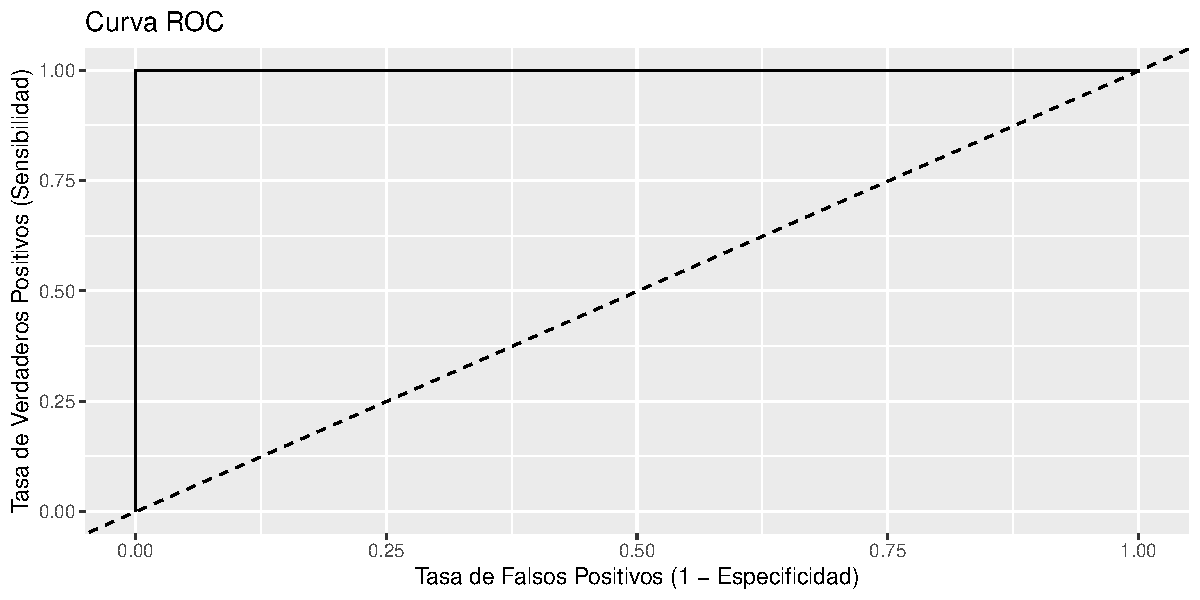
\includegraphics{PRA2_Data_cleaning_and_analysis_files/figure-latex/unnamed-chunk-24-1.pdf}

\begin{Shaded}
\begin{Highlighting}[]
\CommentTok{\# Calcularemos el área debajo de la curva (AUC)}
\NormalTok{auc }\OtherTok{\textless{}{-}} \FunctionTok{auc}\NormalTok{(roc)}

\CommentTok{\# Mostraremos el valor resultante en porcentaje de área abarcada}
\FunctionTok{cat}\NormalTok{(}\StringTok{"Área bajo la curva (AUC): "}\NormalTok{, }\FunctionTok{round}\NormalTok{(auc}\SpecialCharTok{*}\DecValTok{100}\NormalTok{, }\DecValTok{2}\NormalTok{), }\StringTok{"\%"}\NormalTok{)}
\end{Highlighting}
\end{Shaded}

\begin{verbatim}
## Área bajo la curva (AUC):  100 %
\end{verbatim}

La curva es perfecta, con un área del 100\%, corroborando lo expuesto
anteriormente: es un gran modelo.

\hypertarget{resoluciuxf3n-del-problema}{%
\subsection{5. Resolución del
problema}\label{resoluciuxf3n-del-problema}}

\hypertarget{primera-pregunta}{%
\subsubsection{5.1 Primera pregunta}\label{primera-pregunta}}

Para la primera pregunta nos habíamos planteado si un mes de alquiler en
una zona normal es significativamente mayor en Europa que en América.
Para poder responderla, estudiaremos los resultados del análisis por
contraste de hipótesis. Dado que el \textbf{valor observado = 2.964443}
es positivo, todo nos afirma que este valor no está en la zona de
aceptación de la hipótesis nula: (-∞, \(z_{1-∞}\){]}. Por lo tanto,
podemos rechazar la hipótesis nula planteada de igualdad de medias de
alquiler entre Europa y América

Ahora, sabiendo el \textbf{valor \emph{p}} podemos tomar una decisión
sobre las hipótesis. Observando que
\(P(z_{obs}≥2.964443) = 0.001516159\) y nuestro valor de significancia
es \(\alpha = 0.05\), podemos concluir que existe evidencia para
rechazar la hipótesis nula ya que el valor \emph{p} es inferior a 0.05.
Por ende, queda demostrado que el alquiler de un mes en una zona normal
en Europa es significativamente mayor que en América al 95\% de
confianza. Cabe comentar que los países de América incluidos en la
muestra son en su mayoría países de América del Sur, lo cual indica que
los resultados son coherentes.

\hypertarget{segunda-pregunta}{%
\subsubsection{5.2 Segunda pregunta}\label{segunda-pregunta}}

Como hemos comentado podemos ver que el \emph{SMI} de un país podría
determinarse a partir de los datos de gasto mínimo medio en
\emph{Housing} y del \emph{PIB.anual} de un país. Para poder aplicar
este modelo, vamos a considerar los datos de un país que hemos eliminado
del análisis por falta del \emph{SMI} y por un alto \emph{PIB anual}:
\textbf{Singapur}.

\begin{Shaded}
\begin{Highlighting}[]
\CommentTok{\# Datos extraídos de los ficheros de pre{-}procesamiento}
\NormalTok{Housing }\OtherTok{\textless{}{-}} \FloatTok{91.50}
\NormalTok{PIB.anual }\OtherTok{\textless{}{-}} \FloatTok{4.43e12}
\NormalTok{Food }\OtherTok{\textless{}{-}} \DecValTok{15}

\CommentTok{\# creamos el sub{-}dataframe necesario para la predicción}
\NormalTok{df }\OtherTok{\textless{}{-}} \FunctionTok{data.frame}\NormalTok{(}\AttributeTok{Housing =}\NormalTok{ Housing, }\AttributeTok{PIB.anual =}\NormalTok{ PIB.anual, }\AttributeTok{Food =}\NormalTok{ Food)}
\NormalTok{SMI\_Singapur }\OtherTok{\textless{}{-}} \FunctionTok{predict}\NormalTok{(model\_SMI, }\AttributeTok{newdata =}\NormalTok{ df)}

\CommentTok{\# Mostramos la predicción}
\NormalTok{SMI\_Singapur}
\end{Highlighting}
\end{Shaded}

\begin{verbatim}
##        1 
## 1826.059
\end{verbatim}

Por lo tanto, podríamos considerar que el \emph{SMI} de Singapur es
cercano a los 1.826€, lo cuál coincide con los datos recogidos por la
web de
\href{https://www.businesstimes.com.sg/singapore/economy-policy/12000-lower-wage-food-service-workers-earn-least-s1750-mar-1}{\textbf{Business
Times}}

\hypertarget{tercera-pregunta}{%
\subsubsection{5.3 Tercera pregunta}\label{tercera-pregunta}}

Finalmente, solo queda responder la última pregunta. Nos habíamos
cuestionado a que países podríamos ir a trabajar que presenten un SMI
mayor al de España. Como se ha querido asegurar fuertemente que las
predicciones eran correctas, la discretización de las mismas en el
análisis del modelo de regresión logística se llevó a cabo con un nivel
del 80\% de confianza mínimo. Luego, lo único que falta es extraer los
países con predicciones ``superiores al SMI de España'':

\begin{Shaded}
\begin{Highlighting}[]
\CommentTok{\# Creamos un dataframe con las predicciones y los países cuya predicción sea 1}
\NormalTok{predicciones\_df }\OtherTok{\textless{}{-}} \FunctionTok{subset}\NormalTok{(}\FunctionTok{data.frame}\NormalTok{(}\AttributeTok{Country =}\NormalTok{ test\_dataset}\SpecialCharTok{$}\NormalTok{Country, }\AttributeTok{SMI =}\NormalTok{ test\_dataset}\SpecialCharTok{$}\NormalTok{SMI, }\AttributeTok{y\_pred =}\NormalTok{ y\_pred), y\_pred }\SpecialCharTok{==} \DecValTok{1}\NormalTok{)}

\CommentTok{\# Los países candidatos son:}
\NormalTok{predicciones\_df}
\end{Highlighting}
\end{Shaded}

\begin{verbatim}
##        Country    SMI y_pred
## 7  NEW ZEALAND 2156.3      1
## 10      ISRAEL 1528.8      1
\end{verbatim}

\hypertarget{repositorio-github-y-vuxeddeo}{%
\subsection{6. Repositorio Github y
vídeo}\label{repositorio-github-y-vuxeddeo}}

El \emph{link} al repositorio de Github con toda la solución es el
siguiente:\\
\url{https://github.com/Tipologia-y-Ciclo-de-Vida-de-los-Datos/Practica-2--Limpieza-y-Analisis-de-datos}

El vídeo de la práctica se colgará en el apartado de \emph{Video
Práctica} del foro de la asignatura.

\hypertarget{tabla-de-contribuciones}{%
\subsection{Tabla de contribuciones}\label{tabla-de-contribuciones}}

\begin{longtable}[]{@{}ll@{}}
\toprule\noalign{}
CONTRIBUCIONES & FIRMA \\
\midrule\noalign{}
\endhead
\bottomrule\noalign{}
\endlastfoot
Investigación previa & JLSD, MIGS \\
Redacción de las respuestas & JLSD, MIGS \\
Desarrollo del código & JLSD, MIGS \\
Participación en el vídeo & JLSD, MIGS \\
\end{longtable}

\hypertarget{bibliografuxeda}{%
\subsection{Bibliografía}\label{bibliografuxeda}}

\begin{itemize}
\tightlist
\item
  \href{https://datosmacro.expansion.com/divisas}{\textbf{Recurso web:
  Datosmacro}}
\item
  \href{https://materials.campus.uoc.edu/daisy/Materials/PID_00276230/pdf/PID_00276230.pdf}{\textbf{Esteban
  Vega Lozano. Pre procesamiento de los datos}}
\item
  \href{http://materials.cv.uoc.edu/cdocent/PQOAM4CQ8QEFU3ZSSFPQ.pdf}{\textbf{Josep
  Gibergans Baguena. Regresión lineal simple}}
\item
  \href{http://materials.cv.uoc.edu/cdocent/MH1AFH7OY964T7VQCP96.pdf}{\textbf{Josep
  Gibergans Baguena. Regresión lineal múltiple}}
\item
  \href{https://materials.campus.uoc.edu/daisy/Materials/PID_00276229/pdf/PID_00276229.pdf}{\textbf{Montserrat
  Guillén Estany, María Teresa Alonso Alonso. Modelos de regresión
  logística}}
\item
  \href{https://materials.campus.uoc.edu/daisy/Materials/PID_00265704/pdf/PID_00265704.pdf}{\textbf{Laia
  Subirats Maté, Diego Oswaldo Pérez Trenard, Mireia Calvo González.
  Introducción a la limpieza y análisis de los datos}}
\end{itemize}

\end{document}
